% ============================================================
%  RAPPORT PFE — Maintenance Prédictive avec IA
%  Licence en Systèmes Informatiques (LSI) — 2025-2026
%  Compilateur : pdfLaTeX
% ============================================================
\documentclass[12pt, a4paper, oneside]{report}

% ── Bibliographie ────────────────────────────────────────────
\usepackage[numbers]{natbib}

% ── Encodage & langue ────────────────────────────────────────
\usepackage[utf8]{inputenc}
\usepackage[T1]{fontenc}
\usepackage{csquotes}
\usepackage[french]{babel}

% ── Mise en page ─────────────────────────────────────────────
\usepackage[top=2.5cm, bottom=2.5cm, left=3cm, right=2.5cm]{geometry}
\setlength{\headheight}{15pt}
\usepackage{setspace}
\onehalfspacing

% ── Typographie ──────────────────────────────────────────────
\usepackage{lmodern}

% ── Couleurs & graphiques ────────────────────────────────────
\usepackage[dvipsnames, table]{xcolor}
\usepackage{graphicx}
\graphicspath{{image/}{./}{chapters/}}  % cherche dans image/, racine, et chapters/
\usepackage{float}

% ── Tableaux ─────────────────────────────────────────────────
\usepackage{booktabs}
\usepackage{tabularx}
\usepackage{multirow}
\usepackage{longtable}
\usepackage{array}

% ── Listes ───────────────────────────────────────────────────
\usepackage{enumitem}

% ── Liens & PDF ──────────────────────────────────────────────
\usepackage[hidelinks]{hyperref}

% ── En-têtes / pieds de page ─────────────────────────────────
\usepackage{fancyhdr}
\pagestyle{fancy}
\fancyhf{}
\fancyhead[L]{\small\leftmark}
\fancyhead[R]{\small\thepage}
\fancyfoot[C]{\small Système de Maintenance Prédictive avec IA}
\renewcommand{\headrulewidth}{0.4pt}
\renewcommand{\footrulewidth}{0.4pt}

% ── Code source ──────────────────────────────────────────────
\usepackage{listings}
\usepackage{courier}
\definecolor{codebg}{RGB}{245,245,245}
\definecolor{codeframe}{RGB}{200,200,200}
\lstset{
  backgroundcolor=\color{codebg},
  frame=single,
  rulecolor=\color{codeframe},
  basicstyle=\footnotesize\ttfamily,
  breaklines=true,
  captionpos=b,
  numbers=left,
  numberstyle=\tiny\color{gray},
  keywordstyle=\color{blue}\bfseries,
  commentstyle=\color{OliveGreen},
  stringstyle=\color{BrickRed},
  showstringspaces=false,
  tabsize=2
}

% ── Mathématiques ────────────────────────────────────────────
\usepackage{amsmath, amssymb}

% ── Tolérance de mise en page ────────────────────────────────
\sloppy

% ── Numérotation des chapitres ───────────────────────────────
\setcounter{secnumdepth}{3}
\setcounter{tocdepth}{3}

% ── Couleur principale du rapport ────────────────────────────
\definecolor{mainblue}{RGB}{0, 70, 127}
\definecolor{lightblue}{RGB}{220, 235, 250}

% ── Style des titres de chapitres ────────────────────────────
\usepackage{titlesec}
\titleformat{\chapter}[display]
  {\normalfont\huge\bfseries\color{mainblue}}
  {\chaptertitlename\ \thechapter}{20pt}{\Huge}
\titleformat{\section}
  {\normalfont\Large\bfseries\color{mainblue}}
  {\thesection}{1em}{}
\titleformat{\subsection}
  {\normalfont\large\bfseries\color{mainblue!80}}
  {\thesubsection}{1em}{}

% ── Boîtes d'information ─────────────────────────────────────
\usepackage{tcolorbox}
\tcbuselibrary{breakable}
\newtcolorbox{infobox}[1][]{
  colback=lightblue, colframe=mainblue,
  fonttitle=\bfseries, title=#1,
  breakable
}

% ── Acronymes ────────────────────────────────────────────────
\usepackage{acronym}

% ============================================================
\begin{document}

% ── Pages préliminaires (pas de numérotation) ────────────────
\pagenumbering{gobble}

% ============================================================
%  PAGE DE GARDE — Modèle officiel Faculté des Sciences de Gafsa
% ============================================================
\begin{titlepage}
\setlength{\parindent}{0pt}
\setlength{\parskip}{0pt}

% ── TOP: three columns — left text | logo | right text ───────
\noindent
\begin{minipage}[t]{0.35\textwidth}
  \centering\small
  République Tunisienne\\
  Ministère de l'enseignement supérieur\\
  et de la recherche scientifique\\
  Université de Gafsa\\[3pt]
  \textbf{Faculté des Sciences de Gafsa}
\end{minipage}%
\hfill
\begin{minipage}[t]{0.22\textwidth}
  \centering
  \includegraphics[width=3cm]{logo_univ.png}
\end{minipage}%
\hfill
\begin{minipage}[t]{0.35\textwidth}
  \centering\small
  \textbf{Département d'Informatique}\\[4pt]
  Année Universitaire 2024-2025\\[4pt]
  \textbf{Code mémoire :} X/25
\end{minipage}

\vspace{0.5cm}

% ── Department logo ──────────────────────────────────────────
\begin{center}
  \includegraphics[width=8cm]{logo_dept.png}
\end{center}

\vspace{0.3cm}

% ── Main title ───────────────────────────────────────────────
\begin{center}
  {\Large \textbf{MEMOIRE DE PROJET DE FIN D'ETUDES}}\\[0.4cm]
  {\small Présenté en vue de l'obtention du}\\[0.3cm]
  {\normalsize \textbf{DIPLÔME DE LICENCE EN SCIENCES DE L'INFORMATIQUE - LMD}}
\end{center}

\vspace{0.4cm}

% ── Subject block ────────────────────────────────────────────
\begin{center}
  \rule{0.75\linewidth}{1pt}\\[0.3cm]
  {\normalsize Système de Maintenance Prédictive basé sur le Machine Learning}\\[0.3cm]
  \rule{0.75\linewidth}{1pt}
\end{center}

\vspace{0.4cm}

% ── Réalisé par ──────────────────────────────────────────────
\begin{center}
  {\small Réalisé par : \textbf{[Prénom NOM]}}\\[0.15cm]
  {\small et}\\[0.15cm]
  {\small \textbf{[Prénom NOM 2]}}
\end{center}

\vspace{0.25cm}

\begin{center}
  {\small Sous la direction de : \textbf{[Prénom NOM Encadrant]}}
\end{center}

\vspace{0.25cm}

\begin{center}
  {\small Soutenu publiquement le \textbf{---/---/--} devant le jury}
\end{center}

\vspace{0.35cm}

% ── Jury table ───────────────────────────────────────────────
\noindent
\begin{tabular}{@{}ll@{}}
  \textbf{Président :} Mr./Mme. \textbf{[Prénom NOM]}  & \textbf{[Grade]} à l'Université de [Ville] \\[4pt]
  \textbf{Rapporteur :} Mr./Mme. \textbf{[Prénom NOM]} & \textbf{[Grade]} à l'Université de [Ville] \\[4pt]
  \textbf{Encadrant :} Mr./Mme. \textbf{[Prénom NOM]}  & \textbf{[Grade]} à l'Université de [Ville] \\
\end{tabular}

\vfill

% ── Bottom ───────────────────────────────────────────────────
\begin{center}
  $\blacklozenge$ \quad \textbf{Année Universitaire 2024/2025}
\end{center}

\end{titlepage}

% ============================================================
%  REMERCIEMENTS
% ============================================================
\chapter*{Remerciements}
\addcontentsline{toc}{chapter}{Remerciements}
\markboth{Remerciements}{Remerciements}

\vspace{1cm}

Nous tenons à exprimer notre profonde gratitude à toutes les personnes qui ont contribué, de près ou de loin, à la réalisation de ce projet de fin d'études.

\vspace{0.5cm}

Nos remerciements les plus sincères vont en premier lieu à notre encadrant, \textbf{[Prénom NOM]}, pour sa disponibilité, ses précieux conseils et son suivi rigoureux tout au long de ce travail. Ses orientations techniques et méthodologiques ont été déterminantes dans la réussite de ce projet.

\vspace{0.5cm}

Nous remercions également l'ensemble du corps enseignant du département d'informatique pour la qualité de la formation dispensée durant ces trois années de licence, qui nous a fourni les bases nécessaires à la réalisation de ce travail.

\vspace{0.5cm}

Nos remerciements s'adressent aussi aux membres du jury qui ont accepté d'évaluer ce travail et d'enrichir notre réflexion par leurs remarques et suggestions.

\vspace{0.5cm}

Enfin, nous remercions nos familles et amis pour leur soutien moral indéfectible et leurs encouragements constants tout au long de notre parcours académique.

\vspace{1cm}

\begin{flushright}
\textit{L'auteur}
\end{flushright}

% ============================================================
%  DÉDICACE
% ============================================================
\chapter*{Dédicace}
\addcontentsline{toc}{chapter}{Dédicace}
\markboth{Dédicace}{Dédicace}

\vspace{3cm}

\begin{center}
\begin{minipage}{0.75\textwidth}
\begin{center}

\textit{À mes chers parents,}\\[0.5cm]
\textit{pour leur amour inconditionnel, leurs sacrifices et leur soutien sans faille.}\\[0.5cm]
\textit{À mes frères et sœurs,}\\[0.5cm]
\textit{pour leur présence et leurs encouragements.}\\[0.5cm]
\textit{À tous mes amis et collègues,}\\[0.5cm]
\textit{qui ont partagé avec moi les moments difficiles et les réussites.}\\[1cm]

\textit{Je dédie ce modeste travail.}

\end{center}
\end{minipage}
\end{center}


% ── Tables ───────────────────────────────────────────────────
\pagenumbering{roman}
\tableofcontents
\listoffigures
\listoftables

% ── Corps du rapport ─────────────────────────────────────────
\pagenumbering{arabic}

% ============================================================
%  INTRODUCTION GÉNÉRALE
% ============================================================
\chapter*{Introduction Générale}
\addcontentsline{toc}{chapter}{Introduction Générale}
\markboth{Introduction Générale}{Introduction Générale}

\section*{Contexte général}

L'essor de l'intelligence artificielle et de l'apprentissage automatique a profondément
transformé la manière dont les organisations gèrent leurs infrastructures informatiques.
Dans un contexte où la disponibilité des systèmes est devenue un enjeu stratégique majeur,
la maintenance prédictive s'impose comme une approche incontournable pour anticiper les
défaillances matérielles avant qu'elles ne surviennent.

Les parcs informatiques modernes génèrent en permanence des volumes considérables de données
de surveillance : utilisation du processeur, consommation mémoire, état des disques durs,
températures des composants. Ces données, correctement analysées, constituent une source
d'information précieuse pour prédire les pannes et planifier les interventions de maintenance
de manière proactive.

La transformation numérique des entreprises a conduit à une dépendance croissante vis-à-vis
des systèmes informatiques. Une panne non anticipée peut entraîner des pertes financières
considérables, une interruption des services critiques, et une dégradation de la confiance
des utilisateurs. Face à cette réalité, les technologies d'apprentissage automatique offrent
des perspectives prometteuses : les algorithmes de classification, les réseaux de neurones
récurrents et les modèles de détection d'anomalies permettent d'identifier les signes
précurseurs de défaillance bien avant que la panne ne se produise.

\section*{Problématique}

La maintenance réactive, qui consiste à intervenir uniquement après la survenue d'une panne,
engendre des coûts importants : temps d'arrêt non planifiés, perte de productivité, urgences
techniques et remplacement précipité de matériel. La question centrale de ce projet est :

\begin{infobox}[Problématique centrale]
Comment concevoir et implémenter un système intelligent capable de surveiller en temps réel
un parc informatique, d'analyser les tendances des métriques matérielles, et de prédire les
pannes avant qu'elles ne se produisent, afin de permettre une maintenance proactive et
réduire les temps d'arrêt non planifiés ?
\end{infobox}

Cette problématique soulève plusieurs questions secondaires :
\begin{itemize}[leftmargin=1.5cm]
  \item Comment collecter de manière automatique et fiable les métriques système (CPU, RAM,
        disque, SMART) sur un parc hétérogène de machines Windows et Linux ?
  \item Quels algorithmes d'apprentissage automatique sont les plus adaptés à la prédiction
        de défaillances à partir de séries temporelles de métriques système ?
  \item Comment évaluer objectivement la qualité d'un assistant conversationnel spécialisé
        dans le domaine de la maintenance informatique ?
  \item Comment garantir la confidentialité des données d'infrastructure tout en offrant
        des capacités conversationnelles avancées ?
\end{itemize}

\section*{Objectifs du projet}

Ce projet vise à développer une plateforme complète de maintenance prédictive reposant sur
l'intelligence artificielle. Les objectifs principaux sont :

\begin{itemize}[leftmargin=1.5cm]
  \item Mettre en place un agent Python de collecte automatique des métriques système
        (via \texttt{psutil}) et des données SMART (via \texttt{smartctl}) sur chaque
        machine surveillée ;
  \item Concevoir un pipeline d'extraction de 63 caractéristiques statistiques à partir
        des données historiques stockées dans PostgreSQL ;
  \item Entraîner et déployer deux modèles complémentaires : un Random Forest pour les
        métriques système et un LSTM entraîné sur le dataset Backblaze pour les données
        SMART ;
  \item Développer un système d'alertes automatiques par email (Nodemailer/SMTP) pour
        les niveaux de risque HIGH et CRITICAL ;
  \item Créer un tableau de bord React interactif pour la visualisation des métriques,
        des prédictions à 7/14/30 jours, et la gestion des alertes ;
  \item Intégrer un assistant conversationnel hybride basé sur LLaMA 3.2:1b (Ollama)
        fonctionnant entièrement en local, sans transmission de données vers le cloud ;
  \item Évaluer les performances du chatbot avec les métriques ROUGE-1 et ROUGE-2 sur
        un dataset de 20 questions-réponses de référence.
\end{itemize}

\section*{Organisation du rapport}

Ce rapport est organisé en quatre chapitres principaux :

\begin{description}[leftmargin=2cm, style=nextline]
  \item[\textbf{Chapitre 1 — Vue d'ensemble du projet :}] présente le contexte, la
  problématique, les objectifs, la solution proposée et la méthodologie Agile adoptée.

  \item[\textbf{Chapitre 2 — État de l'art :}] passe en revue les fondements théoriques
  de l'apprentissage automatique appliqué à la maintenance prédictive, les modèles LSTM,
  les LLM, et les métriques d'évaluation des systèmes conversationnels.

  \item[\textbf{Chapitre 3 — Conception du système :}] détaille l'architecture
  microservices, la modélisation UML, les besoins fonctionnels et non fonctionnels,
  et les flux de données entre les composants.

  \item[\textbf{Chapitre 4 — Implémentation technique :}] décrit les technologies
  utilisées, l'implémentation de chaque module, les résultats d'évaluation quantitatifs,
  et les captures d'écran de l'interface.
\end{description}

Le rapport se termine par une conclusion générale récapitulant les réalisations et les
perspectives d'évolution du système.

% ============================================================
%  CHAPITRE 1 — VUE D'ENSEMBLE DU PROJET
% ============================================================
\chapter{Vue d'ensemble du projet}

\section{Introduction}

Ce chapitre présente le cadre général du projet de maintenance prédictive avec intelligence
artificielle. Nous y exposons le rôle des agents intelligents dans la surveillance des
systèmes, les limites des approches existantes, les objectifs de notre solution
\textbf{PC Technician Assistant}, ainsi que la méthodologie de développement Agile adoptée
et le planning détaillé des sprints.

\section{Contexte et domaine d'application}

\subsection{Le parc informatique comme actif critique}

Dans les organisations modernes, le parc informatique constitue un actif stratégique dont
la disponibilité conditionne directement la productivité. Un technicien informatique gère
en moyenne entre 50 et 200 postes de travail, serveurs et équipements réseau. La surveillance
manuelle de l'état de santé de chaque machine est non seulement chronophage, mais aussi
insuffisante pour détecter les signes précoces de dégradation.

Les composants les plus sujets aux défaillances dans un parc informatique sont :
\begin{itemize}
  \item \textbf{Les disques durs (HDD/SSD)} : composants soumis à une usure progressive,
        responsables de la majorité des pertes de données non récupérables ;
  \item \textbf{Les processeurs (CPU)} : surchauffe due à une ventilation défaillante ou
        à une charge excessive prolongée, détectable via les capteurs de température ;
  \item \textbf{La mémoire vive (RAM)} : dégradation progressive pouvant entraîner des
        plantages aléatoires et des corruptions de données en mémoire ;
  \item \textbf{Les alimentations électriques} : vieillissement des condensateurs entraînant
        des instabilités de tension difficiles à détecter sans instrumentation.
\end{itemize}

\subsection{Enjeux économiques de la maintenance non planifiée}

Les coûts liés aux pannes informatiques non anticipées sont multidimensionnels. Au-delà du
coût direct du remplacement matériel (majoré de 30 à 50\% en cas d'achat en urgence), les
coûts indirects incluent la perte de productivité des utilisateurs, le temps de récupération
des données, et l'impact sur la continuité de service. La maintenance prédictive vise à
transformer ces coûts réactifs en investissements planifiés et optimisés.

\section{Rôle des agents intelligents dans la surveillance système}

\subsection{Architecture de l'agent de collecte}

Un agent intelligent est un programme autonome capable de percevoir son environnement,
de traiter les informations collectées et d'agir en conséquence. Dans notre système,
l'agent Python est déployé sur chaque machine surveillée et est composé de quatre modules
distincts :

\begin{itemize}
  \item \texttt{collector.py} : collecte les métriques CPU, RAM et disque via \texttt{psutil} ;
  \item \texttt{smart\_reader.py} : lit les attributs SMART du disque via \texttt{smartctl} ;
  \item \texttt{sender.py} : envoie les données au backend avec mécanisme de retry ;
  \item \texttt{scheduler.py} : orchestre la collecte horaire via la bibliothèque
        \texttt{schedule}.
\end{itemize}

\subsection{Métriques collectées par l'agent}

La classe \texttt{SystemCollector} collecte trois catégories de métriques :

\textbf{Métriques CPU :} l'usage est mesuré via \texttt{psutil.cpu\_percent(interval=1)},
qui effectue une mesure sur une seconde pour éviter les valeurs instantanées non
représentatives. La température est lue via \texttt{psutil.sensors\_temperatures()},
avec une recherche séquentielle des capteurs connus (\texttt{coretemp}, \texttt{cpu\_thermal},
\texttt{k10temp}, \texttt{zenpower}). En cas d'indisponibilité des capteurs (fréquent sur
les machines virtuelles), une valeur de fallback de 50°C est utilisée.

\textbf{Métriques mémoire :} \texttt{psutil.virtual\_memory()} retourne le pourcentage
d'utilisation et la mémoire disponible en mégaoctets, calculée par conversion depuis les
octets bruts.

\textbf{Métriques disque :} \texttt{psutil.disk\_usage()} est appelé sur le chemin
\texttt{C:\textbackslash\textbackslash} sous Windows ou \texttt{/} sous Linux, retournant
l'usage en pourcentage et l'espace libre en mégaoctets.

\subsection{Identification unique des machines}

L'identification de chaque machine repose sur une stratégie à trois niveaux de fallback :

\begin{enumerate}
  \item \textbf{Numéro de série BIOS} : via \texttt{wmic bios get serialnumber} (Windows)
        ou \texttt{/sys/class/dmi/id/product\_serial} (Linux). Les valeurs génériques
        (\texttt{TO BE FILLED BY O.E.M.}) sont rejetées ;
  \item \textbf{Adresse MAC} : utilisée si le numéro de série est invalide, formatée
        comme \texttt{MAC-xx:xx:xx:xx:xx:xx} ;
  \item \textbf{Identifiant UUID} : généré via \texttt{uuid.getnode()} comme dernier
        recours, préfixé \texttt{FALLBACK-}.
\end{enumerate}

\subsection{Mécanisme de résilience : retry avec backoff exponentiel}

La classe \texttt{DataSender} implémente un mécanisme de retry robuste pour gérer les
défaillances réseau transitoires. Le comportement est le suivant :

\begin{table}[H]
\centering
\caption{Comportement du mécanisme de retry de l'agent}
\begin{tabular}{|c|c|l|}
\hline
\rowcolor{lightblue}
\textbf{Tentative} & \textbf{Délai d'attente} & \textbf{Condition de déclenchement} \\
\hline
1 & 0s (immédiat) & Première tentative \\
\hline
2 & 1s & Erreur HTTP 5xx ou timeout réseau \\
\hline
3 & 2s & Erreur HTTP 5xx ou timeout réseau \\
\hline
— & Abandon & Erreur HTTP 4xx (erreur client) ou 3 tentatives épuisées \\
\hline
\end{tabular}
\end{table}

Les erreurs 4xx (Bad Request, Unauthorized) ne déclenchent pas de retry car elles indiquent
un problème de configuration (token invalide, payload malformé) qui ne se résoudra pas avec
une nouvelle tentative. Seules les erreurs 5xx (erreurs serveur) et les timeouts réseau
justifient un retry (\texttt{max\_retries = 3}, délais : 1s, 2s).

\section{Problématique et limites des systèmes existants}

\subsection{La maintenance réactive : un modèle dépassé}

La maintenance réactive consiste à intervenir uniquement après la survenue d'une panne.
Ce modèle présente plusieurs inconvénients majeurs :

\begin{itemize}
  \item Temps d'arrêt non planifiés impactant la productivité des utilisateurs ;
  \item Coûts élevés liés aux interventions d'urgence et aux achats de matériel en urgence ;
  \item Risque de perte de données en cas de défaillance soudaine d'un disque dur ;
  \item Impossibilité de planifier les ressources humaines et matérielles à l'avance.
\end{itemize}

\subsection{Limites des outils de monitoring existants}

Des outils comme Nagios, Zabbix ou Datadog offrent des capacités de surveillance en temps
réel basées sur des seuils fixes, mais ne disposent pas de capacités prédictives basées
sur l'apprentissage automatique :

\begin{table}[H]
\centering
\caption{Comparaison des approches de maintenance}
\begin{tabularx}{\textwidth}{|l|X|X|X|}
\hline
\rowcolor{lightblue}
\textbf{Critère} & \textbf{Réactive} & \textbf{Monitoring classique} & \textbf{Notre solution} \\
\hline
Détection & Après panne & Seuils fixes & Prédiction ML \\
\hline
Anticipation & Aucune & Limitée & 7/14/30 jours \\
\hline
ML intégré & Non & Non & Oui (RF + LSTM) \\
\hline
Coût & Élevé & Moyen (500€/mois) & Faible \\
\hline
Données SMART & Non & Partiel & Complet \\
\hline
Chatbot IA & Non & Non & Oui (LLaMA local) \\
\hline
Confidentialité & N/A & Cloud requis & 100\% local \\
\hline
\end{tabularx}
\end{table}

\section{Objectifs et solution proposée}

\subsection{Vision globale : PC Technician Assistant}

Notre solution repose sur quatre piliers fondamentaux :

\begin{enumerate}
  \item \textbf{Collecte automatisée} : un agent Python déployé sur chaque machine collecte
        les métriques système et SMART toutes les heures, de manière transparente ;
  \item \textbf{Prédiction par apprentissage automatique} : deux modèles complémentaires
        (Random Forest sur 63 features statistiques, LSTM sur séquences SMART Backblaze)
        prédisent les pannes à 7, 14 et 30 jours ;
  \item \textbf{Alertes intelligentes} : génération automatique d'alertes par email pour
        les risques HIGH ($\geq 50\%$) et CRITICAL ($\geq 70\%$) ;
  \item \textbf{Interface de gestion} : tableau de bord React avec visualisation des
        métriques, gestion des alertes, et chatbot conversationnel LLaMA local.
\end{enumerate}

\subsection{Niveaux de risque et seuils de décision}

Le système classifie chaque machine selon quatre niveaux de risque basés sur la probabilité
de panne à 30 jours calculée par le modèle Random Forest :

\begin{table}[H]
\centering
\caption{Classification des niveaux de risque et actions associées}
\begin{tabularx}{\textwidth}{|c|c|X|}
\hline
\rowcolor{lightblue}
\textbf{Probabilité (30j)} & \textbf{Niveau} & \textbf{Action déclenchée} \\
\hline
$< 30\%$ & LOW & Surveillance normale, aucune action \\
\hline
$30\% - 50\%$ & MEDIUM & Surveillance accrue, vérification planifiée \\
\hline
$50\% - 70\%$ & HIGH & Création d'alerte + envoi email au technicien \\
\hline
$\geq 70\%$ & CRITICAL & Alerte urgente + email prioritaire \\
\hline
\end{tabularx}
\end{table}

\section{Méthodologie de développement}

\subsection{Approche Agile en quatre sprints}

Le développement a suivi une approche Agile organisée en quatre sprints, chacun produisant
un incrément fonctionnel testable :

\begin{table}[H]
\centering
\caption{Planning des sprints de développement}
\begin{tabularx}{\textwidth}{|c|X|X|}
\hline
\rowcolor{lightblue}
\textbf{Sprint} & \textbf{Période} & \textbf{Livrables principaux} \\
\hline
Sprint 1 & 01 Fév -- 28 Fév 2026 & Agent Python, API Backend Node.js, Base de données PostgreSQL (9 tables), migrations SQL \\
\hline
Sprint 2 & 01 Mar -- 15 Mar 2026 & Dashboard React, Authentification JWT, RBAC Admin/Technicien, composants KPI \\
\hline
Sprint 3 & 16 Mar -- 31 Mar 2026 & Service ML Flask (RF + LSTM), Système d'alertes, Emails SMTP, APScheduler \\
\hline
Sprint 4 & 01 Avr -- 30 Avr 2026 & Chatbot Ollama/LLaMA, Évaluation ROUGE, Docker Compose, Finalisation \\
\hline
\end{tabularx}
\end{table}

\subsection{Gestion du backlog produit}

Le backlog produit a été organisé selon les priorités MoSCoW :

\begin{description}
  \item[\textbf{Must Have (MVP)}] : collecte des métriques, stockage PostgreSQL, prédictions
        Random Forest, alertes email, tableau de bord, authentification JWT ;
  \item[\textbf{Should Have}] : modèle LSTM Backblaze, chatbot IA, export CSV, gestion
        des utilisateurs, versioning des modèles ML ;
  \item[\textbf{Could Have}] : déploiement Docker Compose, évaluation ROUGE, détection
        d'anomalies Isolation Forest ;
  \item[\textbf{Won't Have (v1)}] : application mobile, module de ticketing, rapports PDF.
\end{description}

\section{Conclusion}

Ce chapitre a posé les bases conceptuelles du projet en définissant le problème adressé,
les objectifs visés, l'architecture de l'agent de collecte, et la méthodologie adoptée.
L'approche Agile en quatre sprints a permis de livrer un système complet et fonctionnel
dans les délais impartis. Le chapitre suivant présente l'état de l'art des technologies
utilisées, notamment les modèles d'apprentissage automatique pour la maintenance prédictive
et les approches d'évaluation des systèmes conversationnels.

% ============================================================
%  CHAPITRE 2 — ÉTAT DE L'ART
% ============================================================
\chapter{État de l'art}

\section{Introduction}

Ce chapitre présente les fondements théoriques sur lesquels repose notre système de
maintenance prédictive. Nous abordons successivement les stratégies de maintenance,
la technologie SMART, les algorithmes d'apprentissage automatique utilisés (Random
Forest, Isolation Forest, LSTM), les modèles de langage de grande taille (LLM), et
les métriques d'évaluation des systèmes conversationnels.

% ─────────────────────────────────────────────────────────────
\section{Maintenance prédictive — Contexte et enjeux}
% ─────────────────────────────────────────────────────────────

\subsection{Évolution des stratégies de maintenance}

La maintenance des équipements informatiques a évolué à travers trois générations
\cite{mobley2002maintenance} :

\begin{description}
  \item[\textbf{Maintenance corrective (réactive)}] : on intervient uniquement après
  la panne. Cette approche est coûteuse en temps d'arrêt et en ressources humaines,
  et ne permet aucune anticipation.

  \item[\textbf{Maintenance préventive (planifiée)}] : les interventions sont
  programmées à intervalles fixes, indépendamment de l'état réel de l'équipement.
  Cela peut entraîner des remplacements prématurés ou des pannes entre deux
  interventions planifiées.

  \item[\textbf{Maintenance prédictive (conditionnelle)}] : l'état réel de
  l'équipement est surveillé en continu. On n'intervient que lorsque des signes de
  dégradation sont détectés. Cette approche optimise les coûts et réduit les temps
  d'arrêt non planifiés.
\end{description}

\subsection{Données SMART — Self-Monitoring, Analysis and Reporting Technology}

La technologie SMART est intégrée dans la quasi-totalité des disques durs modernes
depuis les années 1990. Elle permet de surveiller en temps réel l'état de santé du
disque à travers une série d'attributs normalisés. Dans notre système, le module
\texttt{SmartReader} utilise \texttt{smartctl} pour lire ces attributs sur Windows
et Linux.

\begin{table}[H]
\centering
\caption{Principaux attributs SMART utilisés dans le projet}
\begin{tabularx}{\textwidth}{|c|l|X|}
\hline
\rowcolor{lightblue}
\textbf{ID} & \textbf{Nom} & \textbf{Rôle dans notre système} \\
\hline
5   & Reallocated Sectors Count & Mappé sur \texttt{read\_errors} \\
\hline
187 & Reported Uncorrectable Errors & Mappé sur \texttt{write\_errors} \\
\hline
194 & Temperature Celsius & Mappé sur \texttt{temperature} \\
\hline
197 & Current Pending Sector Count & Contribue au \texttt{health\_score} LSTM \\
\hline
198 & Offline Uncorrectable & Contribue au \texttt{health\_score} LSTM \\
\hline
\end{tabularx}
\end{table}

Des études ont montré que les attributs 5, 187, 197 et 198 sont les meilleurs
prédicteurs de défaillance imminente d'un disque dur \cite{backblaze2020,
pinheiro2007smart}. Notre modèle LSTM exploite précisément ces attributs, mappés
depuis le dataset Backblaze vers notre schéma de base de données.

Lorsque \texttt{smartctl} n'est pas disponible (machines virtuelles, conteneurs),
l'agent utilise des valeurs de fallback : \texttt{health\_status = GOOD},
\texttt{read\_errors = 0}, \texttt{write\_errors = 0}, \texttt{temperature = 40°C}.
Cela garantit que la collecte continue même sur des environnements sans accès SMART.

% ─────────────────────────────────────────────────────────────
\section{Apprentissage automatique pour la maintenance prédictive}
% ─────────────────────────────────────────────────────────────

\subsection{Formulation du problème}

La prédiction de panne est traitée comme un problème de \textbf{classification
binaire} : à partir des métriques historiques d'une machine sur les 30 derniers
jours, le modèle prédit si une panne est probable dans un horizon de 7, 14 ou
30 jours. La sortie est une probabilité entre 0 et 100\%, convertie ensuite en
niveau de risque (LOW / MEDIUM / HIGH / CRITICAL).

\subsection{Random Forest}

Le Random Forest \cite{breiman2001rf} est un algorithme d'ensemble qui combine
plusieurs arbres de décision entraînés sur des sous-ensembles aléatoires des
données. La prédiction finale est obtenue par vote majoritaire entre tous les
arbres. Plus un arbre vote pour la classe « panne », plus la probabilité estimée
est élevée.

\textbf{Pourquoi ce choix pour notre projet :}
\begin{itemize}
  \item Robuste aux valeurs aberrantes et aux données manquantes ;
  \item Fournit un score d'importance pour chaque feature, affiché dans le
        composant \texttt{MachineDetails} du frontend ;
  \item Performant sur les données tabulaires sans nécessiter de GPU ;
  \item Gère nativement les classes déséquilibrées via le paramètre
        \texttt{class\_weight='balanced'} ;
  \item Facile à versionner et à comparer entre cycles d'entraînement.
\end{itemize}

\textbf{Hyperparamètres retenus :}
\begin{table}[H]
\centering
\caption{Hyperparamètres du Random Forest}
\begin{tabularx}{\textwidth}{|l|c|X|}
\hline
\rowcolor{lightblue}
\textbf{Paramètre} & \textbf{Valeur} & \textbf{Justification} \\
\hline
\texttt{n\_estimators} & 100 & Bon compromis précision / temps de calcul \\
\hline
\texttt{max\_depth} & 10 & Évite l'overfitting sur 63 features \\
\hline
\texttt{min\_samples\_split} & 5 & Régularisation des nœuds internes \\
\hline
\texttt{class\_weight} & balanced & Compense la rareté des pannes dans les données \\
\hline
\texttt{random\_state} & 42 & Reproductibilité des résultats \\
\hline
\end{tabularx}
\end{table}

\subsection{Isolation Forest pour la détection d'anomalies}

L'Isolation Forest \cite{liu2008isolation} est un algorithme non supervisé de
détection d'anomalies. Son principe est simple : les observations anormales sont
rares et différentes des observations normales, donc elles sont plus faciles à
isoler. L'algorithme construit des arbres aléatoires et mesure combien d'étapes
sont nécessaires pour isoler chaque point — moins il en faut, plus le point est
anormal.

Dans notre système, l'Isolation Forest est configuré avec 10\% d'anomalies
attendues (\texttt{contamination = 0.1}). Il opère sur les mêmes 63 features que
le Random Forest, mais de manière non supervisée, ce qui permet de détecter des
comportements inhabituels même sans historique de pannes.

\subsection{Ingénierie des caractéristiques (Feature Engineering)}

L'extraction de caractéristiques pertinentes est une étape cruciale du pipeline ML.
La classe \texttt{FeatureExtractor} extrait \textbf{63 caractéristiques} par machine
à partir des 30 derniers jours de données stockées dans PostgreSQL.

\begin{table}[H]
\centering
\caption{Les 63 caractéristiques extraites par \texttt{FeatureExtractor}}
\begin{tabularx}{\textwidth}{|c|l|X|}
\hline
\rowcolor{lightblue}
\textbf{Nb} & \textbf{Type} & \textbf{Description} \\
\hline
45 & Statistiques glissantes & Moyenne, médiane, écart-type, min, max sur 3 métriques
     $\times$ 3 fenêtres (24h, 168h, 720h) \\
\hline
3  & Tendances & Pente de la droite de régression sur 7 jours (via \texttt{numpy.polyfit}) \\
\hline
3  & Taux de variation & Différence entre la valeur courante et la valeur de l'heure précédente \\
\hline
3  & Volatilité & Coefficient de variation (écart-type / moyenne) \\
\hline
6  & SMART & Température, erreurs lecture/écriture, statut de santé (encodage one-hot) \\
\hline
3  & Temporel & Heure de la journée, jour de la semaine, indicateur week-end \\
\hline
\end{tabularx}
\end{table}

Les fenêtres temporelles de 24h, 168h (7 jours) et 720h (30 jours) permettent au
modèle de capturer à la fois les variations à court terme et les tendances de
dégradation à long terme. Les valeurs manquantes sont traitées par forward-fill
(propagation de la dernière valeur connue, limitée à 3 points consécutifs), puis
remplacement par zéro.

% ─────────────────────────────────────────────────────────────
\section{Réseaux de neurones récurrents et LSTM}
% ─────────────────────────────────────────────────────────────

\subsection{Réseaux de neurones récurrents (RNN)}

Les RNN sont conçus pour traiter des séquences de données en conservant une
mémoire des pas de temps précédents. Contrairement aux réseaux classiques, ils
maintiennent un état interne qui se met à jour à chaque nouvelle entrée. Cependant,
les RNN classiques ont du mal à mémoriser des informations sur de longues séquences
— c'est le problème de la disparition du gradient.

\subsection{Long Short-Term Memory (LSTM)}

Le LSTM \cite{hochreiter1997lstm} résout ce problème grâce à un mécanisme de
\textbf{portes} qui contrôle sélectivement ce que le réseau doit mémoriser, oublier
ou transmettre :

\begin{itemize}
  \item \textbf{Porte d'oubli} : décide quelle information de l'état précédent
        doit être effacée ;
  \item \textbf{Porte d'entrée} : décide quelle nouvelle information doit être
        mémorisée ;
  \item \textbf{Porte de sortie} : décide quelle partie de la mémoire doit être
        transmise comme sortie.
\end{itemize}

Ce mécanisme permet au LSTM de capturer des dépendances à long terme dans les
séquences de métriques SMART, comme une augmentation progressive des erreurs sur
plusieurs jours précédant une panne.

\subsection{Architecture LSTM dans notre projet}

Notre modèle PyTorch (\texttt{lstm\_predictor.py}) analyse des séquences de
\textbf{5 mesures SMART consécutives} pour prédire la probabilité de défaillance
d'un disque. L'architecture est volontairement simple et légère :

\begin{itemize}
  \item \textbf{Entrée} : séquence de 5 pas de temps, chacun avec 4 valeurs :
        \texttt{read\_errors}, \texttt{write\_errors}, \texttt{temperature},
        \texttt{health\_score} ;
  \item \textbf{Couche LSTM} : 32 unités cachées ;
  \item \textbf{Couche de sortie} : une valeur entre 0 et 1 (probabilité de panne),
        obtenue via une activation sigmoïde.
\end{itemize}

Le \texttt{health\_score} est un encodage numérique du statut SMART :
0,0 pour GOOD, 0,5 pour WARNING, 1,0 pour CRITICAL. Les quatre features sont
normalisées par des valeurs maximales fixes avant d'être passées au modèle, ce
qui évite les sorties saturées.

\subsection{Dataset Backblaze}

Le dataset Backblaze est une référence dans le domaine de la prédiction de
défaillance des disques durs. Backblaze publie trimestriellement les données SMART
de ses disques en production, avec les événements de panne réels documentés.

Pour le Q1 2020, le dataset utilisé dans notre projet contient :
\begin{itemize}
  \item 874 892 lignes de données SMART réelles ;
  \item 4 993 disques uniques ;
  \item 9 981 séquences temporelles construites (fenêtre glissante de 5 jours) ;
  \item Des pannes réelles documentées (colonne \texttt{failure} = 1).
\end{itemize}

\textbf{Correspondance des attributs Backblaze vers notre schéma :}

\begin{table}[H]
\centering
\caption{Mapping des attributs Backblaze vers les features LSTM}
\begin{tabular}{|l|l|l|}
\hline
\rowcolor{lightblue}
\textbf{Attribut Backblaze} & \textbf{Signification SMART} & \textbf{Feature projet} \\
\hline
\texttt{smart\_5\_raw} & Reallocated Sectors Count & \texttt{read\_errors} \\
\hline
\texttt{smart\_187\_raw} & Reported Uncorrectable Errors & \texttt{write\_errors} \\
\hline
\texttt{smart\_194\_raw} & Temperature Celsius & \texttt{temperature} \\
\hline
\texttt{smart\_197\_raw} + \texttt{smart\_198\_raw} & Pending + Uncorrectable Sectors & \texttt{health\_score} \\
\hline
\end{tabular}
\end{table}

\subsection{Gestion du déséquilibre de classes}

Le dataset Backblaze est fortement déséquilibré : les pannes représentent moins
de 1\% des enregistrements. Trois techniques sont combinées pour gérer ce problème :

\begin{enumerate}
  \item \textbf{Oversampling} : les séquences de panne sont dupliquées jusqu'à
        représenter 10\% du dataset d'entraînement ;
  \item \textbf{Pondération de la loss} : la fonction de perte pénalise 50 fois
        plus fortement les pannes manquées que les fausses alarmes ;
  \item \textbf{Réduction progressive du learning rate} : le taux d'apprentissage
        est divisé par 2 tous les 7 epochs pour stabiliser la convergence.
\end{enumerate}

% ─────────────────────────────────────────────────────────────
\section{Modèles de langage de grande taille (LLM)}
% ─────────────────────────────────────────────────────────────

\subsection{Architecture Transformer}

Les LLM modernes reposent sur l'architecture Transformer \cite{vaswani2017attention},
qui utilise un mécanisme d'\textbf{attention} pour pondérer l'importance de chaque
mot dans une phrase par rapport aux autres. Contrairement aux RNN, le Transformer
traite tous les mots en parallèle, ce qui le rend beaucoup plus rapide à entraîner
et capable de capturer des relations à très longue portée dans le texte.

\subsection{Ollama et LLaMA 3.2:1b}

Ollama est un framework permettant d'exécuter des LLM localement, sans connexion
internet ni GPU dédié \cite{touvron2023llama}. Dans notre projet, nous utilisons
\textbf{LLaMA 3.2:1b} (1 milliard de paramètres), qui offre un bon compromis entre
qualité des réponses et vitesse d'inférence sur du matériel standard.

Le choix d'un LLM local est motivé par la \textbf{confidentialité} : aucune donnée
sur l'infrastructure (noms de machines, métriques, alertes) n'est transmise à des
services cloud tiers.

\textbf{Paramètres d'inférence configurés :}
\begin{itemize}
  \item \texttt{temperature = 0.3} : réponses cohérentes et reproductibles,
        évitant les hallucinations sur des données techniques ;
  \item \texttt{num\_predict = 150} : limite la longueur des réponses pour
        la rapidité ;
  \item \texttt{repeat\_penalty = 1.1} : évite les répétitions dans les réponses.
\end{itemize}

% ─────────────────────────────────────────────────────────────
\section{Métriques d'évaluation}
% ─────────────────────────────────────────────────────────────

\subsection{ROUGE pour l'évaluation du chatbot}

ROUGE (\textit{Recall-Oriented Understudy for Gisting Evaluation})
\cite{lin2004rouge} est une famille de métriques qui mesure le chevauchement
lexical entre une réponse générée et une réponse de référence. Plus les mots
en commun sont nombreux, plus le score est élevé.

Notre pipeline d'évaluation (\texttt{evaluate.py}) calcule deux variantes :
\begin{itemize}
  \item \textbf{ROUGE-1} : chevauchement des mots individuels (unigrammes) ;
  \item \textbf{ROUGE-2} : chevauchement des paires de mots consécutifs (bigrammes).
\end{itemize}

Le score F1 est utilisé, qui équilibre précision (mots générés corrects) et rappel
(mots de référence retrouvés). La bibliothèque \texttt{rouge-score} est utilisée
avec \texttt{use\_stemmer=True} pour normaliser les formes fléchies en français.

\subsection{Métriques de classification pour les modèles ML}

\begin{table}[H]
\centering
\caption{Métriques d'évaluation des modèles de classification}
\begin{tabularx}{\textwidth}{|l|X|l|}
\hline
\rowcolor{lightblue}
\textbf{Métrique} & \textbf{Signification} & \textbf{Formule simplifiée} \\
\hline
Accuracy & Proportion de prédictions correctes & (TP + TN) / Total \\
\hline
Précision & Parmi les pannes prédites, combien sont réelles & TP / (TP + FP) \\
\hline
Rappel & Parmi les vraies pannes, combien sont détectées & TP / (TP + FN) \\
\hline
F1-Score & Équilibre entre précision et rappel & 2 $\times$ P $\times$ R / (P + R) \\
\hline
ROC AUC & Capacité discriminante globale du modèle & Aire sous la courbe ROC \\
\hline
\end{tabularx}
\end{table}

Dans le contexte de la maintenance prédictive, le \textbf{rappel} est la métrique
la plus critique : manquer une vraie panne (faux négatif) est bien plus coûteux
qu'une fausse alarme (faux positif). C'est pourquoi notre LSTM est configuré pour
maximiser le rappel, atteignant 100\% sur le dataset Backblaze.

% ─────────────────────────────────────────────────────────────
\section{Travaux connexes}
% ─────────────────────────────────────────────────────────────

Plusieurs travaux académiques ont abordé la prédiction de défaillance des disques
durs à partir des données SMART. \cite{lei2018machinery} présente une revue
complète des applications du ML à la maintenance prédictive industrielle. Les
approches basées sur les données Backblaze ont montré que les attributs SMART 5,
187, 197 et 198 sont les plus prédictifs de défaillance imminente, avec des
précisions allant de 85\% à 95\% selon les modèles \cite{pinheiro2007smart}.

Notre contribution se distingue par l'intégration d'un pipeline complet de bout
en bout : de la collecte automatisée des données jusqu'à l'interface
conversationnelle, en passant par deux modèles ML complémentaires (Random Forest
pour les métriques système agrégées et LSTM pour les séquences temporelles SMART),
le tout déployé en microservices Docker.

% ─────────────────────────────────────────────────────────────
\section{Conclusion}
% ─────────────────────────────────────────────────────────────

Cet état de l'art a présenté les fondements théoriques des technologies utilisées
dans notre projet. Le Random Forest et le LSTM constituent des approches
complémentaires pour la prédiction de pannes : le premier opère sur 63
caractéristiques statistiques agrégées sur 30 jours, le second capture les
dynamiques temporelles de dégradation des disques sur des séquences de 5 mesures
SMART. Les métriques ROUGE permettent d'évaluer objectivement la qualité du
chatbot sur un dataset de 20 questions de référence. Le chapitre suivant détaille
la conception architecturale du système.

% ============================================================
%  CHAPITRE 3 — CONCEPTION DU SYSTÈME
% ============================================================
\chapter{Conception du système}

\section{Introduction}

Ce chapitre présente la conception architecturale complète du système de maintenance
prédictive. Nous détaillons les besoins fonctionnels et non fonctionnels, la modélisation
UML à travers cinq diagrammes, l'architecture microservices, le schéma de la base de
données, et les flux de données entre les composants.

La conception a été guidée par trois principes fondamentaux : la \textbf{séparation des
responsabilités} entre les services (chaque service a un rôle unique et bien défini),
la \textbf{résilience} face aux pannes réseau (retry exponentiel, verrous distribués),
et la \textbf{scalabilité} pour supporter un nombre croissant de machines surveillées.

% ─────────────────────────────────────────────────────────────
\section{Besoins fonctionnels}
% ─────────────────────────────────────────────────────────────

Les besoins fonctionnels ont été identifiés à partir de l'analyse des cas d'utilisation
et des entretiens avec les utilisateurs cibles (techniciens informatiques et administrateurs
système). Ils sont organisés par module fonctionnel :

\begin{table}[H]
\centering
\caption{Besoins fonctionnels du système}
\begin{tabularx}{\textwidth}{|c|l|X|}
\hline
\rowcolor{lightblue}
\textbf{ID} & \textbf{Fonctionnalité} & \textbf{Description} \\
\hline
BF01 & Collecte automatique & L'agent collecte CPU, RAM, disque et SMART toutes les heures \\
\hline
BF02 & Authentification & Connexion sécurisée par JWT avec rôles Admin/Technicien \\
\hline
BF03 & Prédiction ML & Calcul de la probabilité de panne à 7, 14 et 30 jours \\
\hline
BF04 & Alertes automatiques & Création d'alertes et envoi d'emails pour risques HIGH/CRITICAL \\
\hline
BF05 & Tableau de bord & Visualisation des métriques, prédictions RF (Proba. Panne) et LSTM (Santé Disque) côte à côte, et alertes \\
\hline
BF06 & Gestion des alertes & Accusé de réception et résolution des alertes \\
\hline
BF07 & Chatbot IA & Assistant conversationnel en langage naturel \\
\hline
BF08 & Gestion utilisateurs & Création, modification et suppression de comptes (Admin) \\
\hline
BF09 & Export CSV & Export des données de métriques au format CSV \\
\hline
BF10 & Détection d'anomalies & Isolation Forest pour détecter les comportements anormaux \\
\hline
BF11 & Prédiction LSTM & Prédiction de défaillance disque via le modèle LSTM Backblaze \\
\hline
BF12 & Versioning modèles & Registre des modèles ML avec activation conditionnelle \\
\hline
\end{tabularx}
\end{table}

% ─────────────────────────────────────────────────────────────
\section{Besoins non fonctionnels}
% ─────────────────────────────────────────────────────────────

\begin{table}[H]
\centering
\caption{Besoins non fonctionnels du système}
\begin{tabularx}{\textwidth}{|l|X|}
\hline
\rowcolor{lightblue}
\textbf{Critère} & \textbf{Exigence} \\
\hline
Performance & Temps de réponse API $<$ 100ms, requêtes DB $<$ 50ms \\
\hline
Disponibilité & Collecte automatique 24h/24, prédictions quotidiennes à 2h00 \\
\hline
Sécurité & JWT (24h), bcrypt (10 rounds), protection injection SQL via ORM Sequelize \\
\hline
Scalabilité & Architecture microservices permettant le déploiement indépendant de chaque service \\
\hline
Fiabilité & Retry exponentiel pour l'agent, verrou distribué PostgreSQL pour le scheduler \\
\hline
Confidentialité & LLM local (Ollama), aucune donnée transmise à des services cloud \\
\hline
Maintenabilité & Code modulaire, versioning des modèles ML, logs rotatifs \\
\hline
Portabilité & Conteneurisation Docker, compatible Windows et Linux \\
\hline
\end{tabularx}
\end{table}

% ─────────────────────────────────────────────────────────────
\section{Diagramme de classes}
% ─────────────────────────────────────────────────────────────

\subsection{Description}

Le diagramme de classes représente la structure statique du système. L'entité centrale
est \textbf{Machine}, qui est associée à plusieurs types de données collectées
(\texttt{SystemMetrics}, \texttt{SmartData}), aux résultats d'analyse (\texttt{Prediction},
\texttt{Anomaly}), et aux notifications générées (\texttt{Alert}). Les modèles ML sont
versionnés dans \texttt{MLModel}. Les utilisateurs sont gérés via \texttt{User} avec un
système de rôles (Admin / Viewer).

\subsection{Diagramme}

\begin{figure}[H]
  \centering
  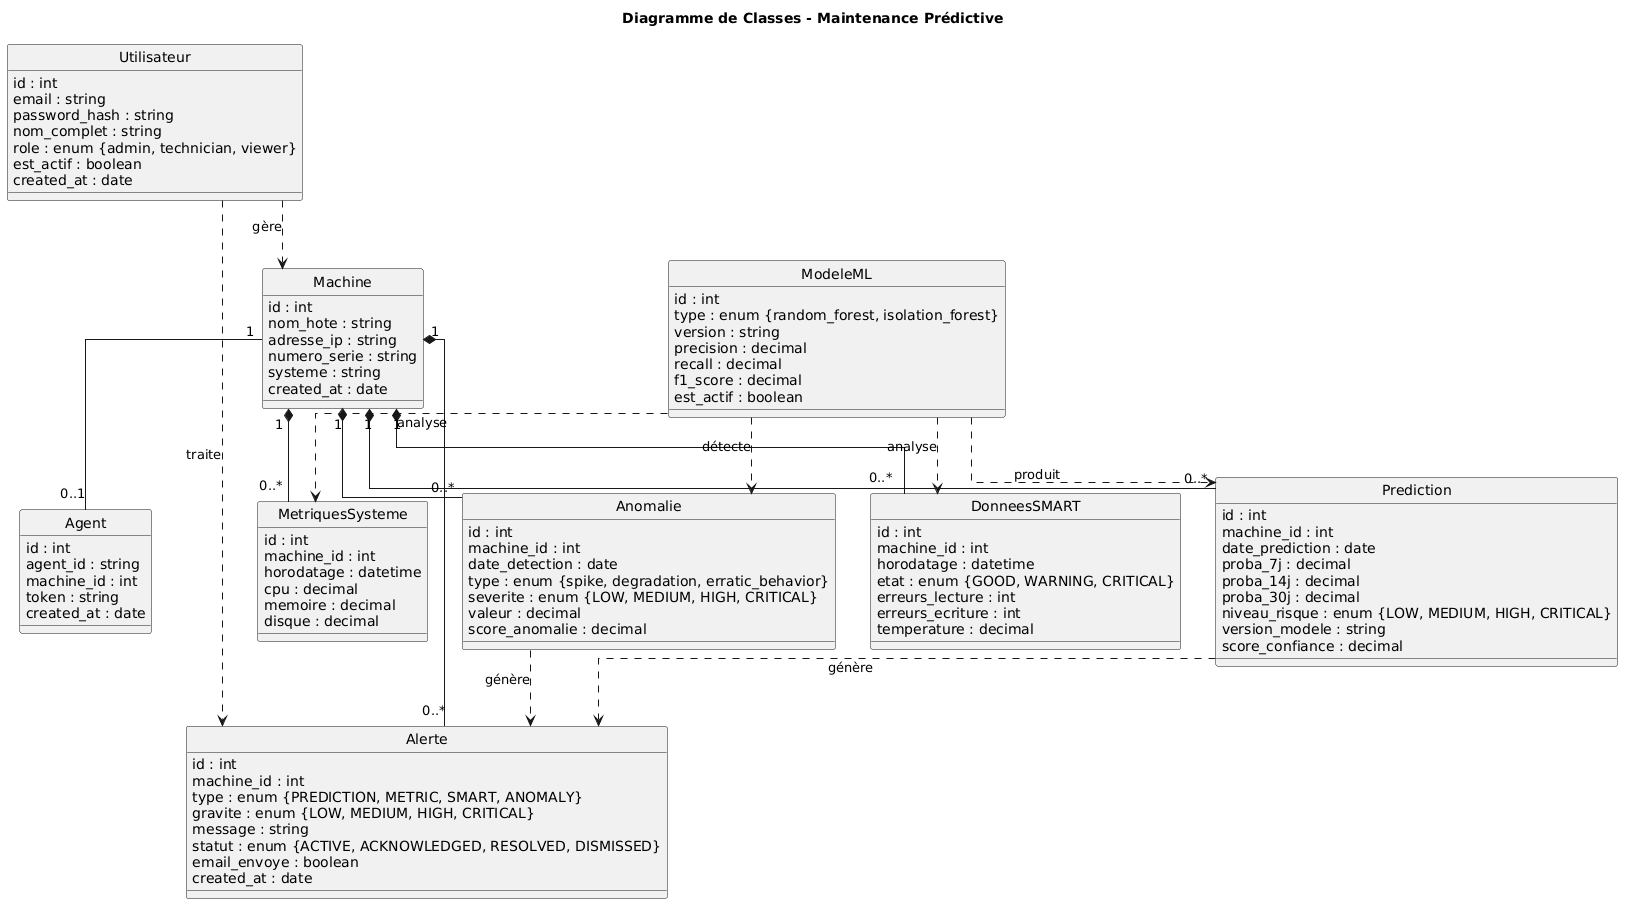
\includegraphics[width=0.95\textwidth]{class_diagram.png}
  \caption{Diagramme de classes du système}
\end{figure}

\subsection{Interprétation des relations}

Ce diagramme illustre les relations suivantes :
\begin{itemize}
  \item Une \textbf{Machine} génère plusieurs \texttt{SystemMetrics}
        (relation 1..* — collecte horaire via l'agent) ;
  \item Une \textbf{Machine} possède plusieurs \texttt{SmartData}
        (données SMART du disque dur, collectées simultanément) ;
  \item Une \textbf{Machine} est associée à plusieurs \texttt{Prediction}
        (historique des prédictions ML générées chaque nuit à 2h00) ;
  \item Une \textbf{Machine} peut générer plusieurs \texttt{Alert}
        (alertes HIGH/CRITICAL avec statut ACTIVE/ACKNOWLEDGED/RESOLVED) ;
  \item Un \textbf{MLModel} est référencé par les \texttt{Prediction} via
        \texttt{model\_version}, permettant de tracer quelle version du modèle
        a produit chaque prédiction.
\end{itemize}

Les données collectées par l'agent (\texttt{SystemMetrics} et \texttt{SmartData}) sont
utilisées par les modèles de machine learning pour détecter les anomalies et générer les
prédictions. Si un problème est détecté (probabilité de panne $\geq 50\%$), le système
crée automatiquement une \texttt{Alert} et envoie une notification par email.

% ─────────────────────────────────────────────────────────────
\section{Diagramme de cas d'utilisation}
% ─────────────────────────────────────────────────────────────

\subsection{Description}

Le diagramme de cas d'utilisation identifie quatre acteurs dans le système :
\begin{itemize}
  \item \textbf{Administrateur} : gère les utilisateurs, les machines et a accès à toutes
        les fonctionnalités du système ;
  \item \textbf{Technicien} : surveille le système via le tableau de bord, gère les alertes,
        consulte les prédictions et interagit avec le chatbot ;
  \item \textbf{Agent de collecte} : programme Python autonome qui collecte et envoie les
        données automatiquement toutes les heures ;
  \item \textbf{Système ML} : service automatique qui génère les prédictions et déclenche
        les alertes sans intervention humaine.
\end{itemize}

\subsection{Diagramme}

\begin{figure}[H]
  \centering
  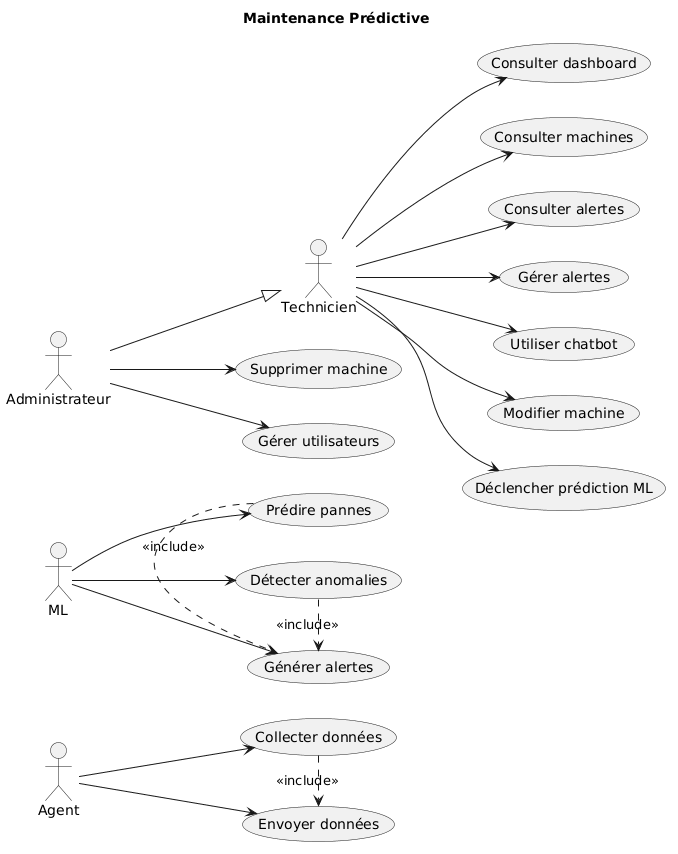
\includegraphics[width=0.95\textwidth]{use_case_diagram.png}
  \caption{Diagramme de cas d'utilisation}
\end{figure}

\subsection{Interprétation}

L'administrateur dispose de tous les droits, y compris la gestion des utilisateurs
(création, modification de rôle, suppression via le middleware \texttt{requireAdmin}).
Le technicien a un accès fonctionnel : il peut consulter le tableau de bord, visualiser
les détails des machines, gérer les alertes (accusé de réception, résolution) et interagir
avec le chatbot. L'agent de collecte et le système ML sont des acteurs automatiques qui
n'interagissent pas directement avec l'interface utilisateur.

% ─────────────────────────────────────────────────────────────
\section{Diagramme de séquence — Affichage du tableau de bord}
% ─────────────────────────────────────────────────────────────

\subsection{Description}

Ce diagramme illustre le flux d'interactions lors de l'ouverture du tableau de bord par
un technicien. L'utilisateur s'authentifie, le frontend envoie une requête au backend,
qui interroge la base de données et retourne les données agrégées (KPIs, liste des
machines, alertes actives).

\subsection{Diagramme}

\begin{figure}[H]
  \centering
  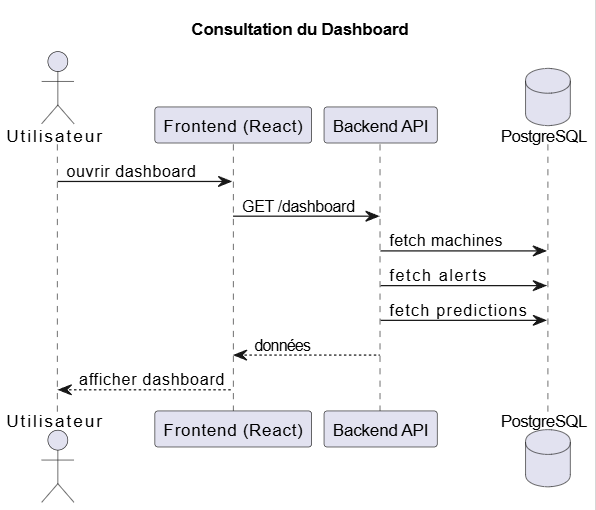
\includegraphics[width=0.95\textwidth]{sequence_dashboard.png}
  \caption{Diagramme de séquence — Affichage du tableau de bord}
\end{figure}

\subsection{Interprétation}

Le flux commence par l'authentification de l'utilisateur qui reçoit un token JWT signé
avec \texttt{JWT\_SECRET}, valide 24 heures. Ce token est inclus dans toutes les requêtes
suivantes dans l'en-tête \texttt{Authorization: Bearer <token>}. Le backend effectue deux
requêtes SQL principales : une pour les KPIs globaux (nombre de machines, alertes actives,
risque moyen) via \texttt{GET /api/dashboard/overview}, et une pour la liste complète des
machines avec leurs dernières prédictions RF et LSTM via \texttt{GET /api/dashboard/machines}.
Le frontend React reçoit les données JSON et effectue le rendu des composants (\texttt{KPICards},
\texttt{MachineList}, \texttt{AlertsList}), le composant \texttt{MachineList} affichant
notamment deux colonnes de prédiction distinctes : ``Proba. Panne (RF)'' et ``Santé Disque (LSTM)''.
Le temps de réponse total est inférieur à 100ms.

% ─────────────────────────────────────────────────────────────
\section{Diagramme de séquence — Génération de prédictions}
% ─────────────────────────────────────────────────────────────

\subsection{Description}

Ce diagramme illustre le pipeline de prédiction automatique déclenché chaque nuit à 2h00.
Le scheduler APScheduler réveille le service ML, qui extrait les caractéristiques, applique
le modèle Random Forest, calcule le niveau de risque, et génère les alertes si nécessaire.

\subsection{Diagramme}

\begin{figure}[H]
  \centering
  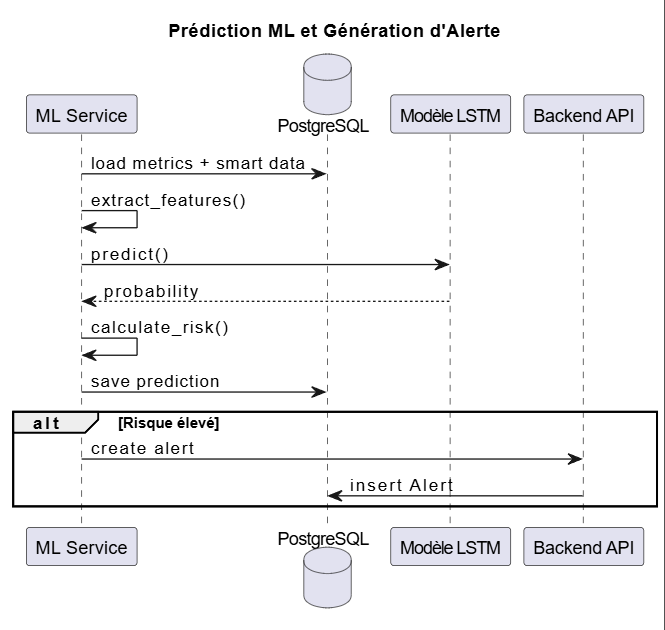
\includegraphics[width=0.95\textwidth]{sequence_prediction_alert.png}
  \caption{Diagramme de séquence — Génération de prédictions et alertes}
\end{figure}

\subsection{Interprétation}

Le pipeline commence par l'acquisition d'un verrou distribué PostgreSQL
(\texttt{pg\_try\_advisory\_lock(12345)}) pour éviter les exécutions concurrentes en cas
de redémarrage du service. Le service ML extrait ensuite 63 caractéristiques statistiques
sur les 30 derniers jours pour chaque machine. Le modèle Random Forest actif (récupéré
depuis le registre \texttt{ml\_models}) calcule la probabilité de panne. Si le risque est
HIGH ($\geq 50\%$) ou CRITICAL ($\geq 70\%$), une alerte est créée dans la base de données
et un email HTML est envoyé via SMTP (Nodemailer). Le verrou est libéré à la fin du
traitement. En cas d'échec, un retry est planifié 1 heure plus tard.

% ─────────────────────────────────────────────────────────────
\section{Diagramme de séquence — Collecte de données}
% ─────────────────────────────────────────────────────────────

\subsection{Description}

Ce diagramme illustre le cycle de collecte horaire de l'agent Python. L'agent collecte
les métriques système et SMART, construit le payload JSON, et l'envoie au backend avec
un mécanisme de retry en cas d'échec.

\subsection{Diagramme}

\begin{figure}[H]
  \centering
  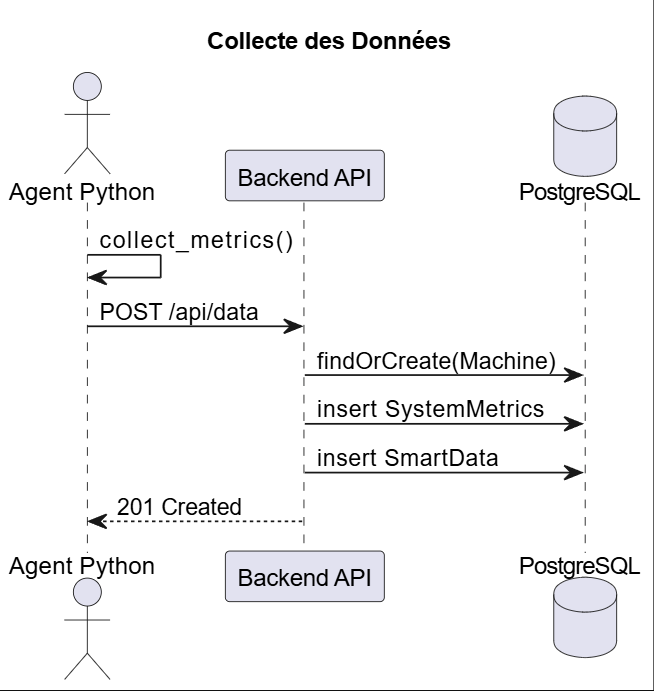
\includegraphics[width=0.95\textwidth]{sequence_data_collection.png}
  \caption{Diagramme de séquence — Collecte de données par l'agent}
\end{figure}

\subsection{Interprétation}

L'agent exécute un cycle de collecte complet toutes les heures. Il collecte
séquentiellement les métriques CPU (usage + température), RAM (usage + disponible),
disque (usage + libre), puis les données SMART via \texttt{smartctl}. Si SMART n'est
pas disponible sur le matériel, des valeurs par défaut sont utilisées. Le payload JSON
est envoyé au backend avec un token Bearer. En cas d'erreur serveur (5xx), l'agent
réessaie avec un backoff exponentiel (1s, 2s, 4s). Les erreurs client (4xx) ne
déclenchent pas de retry.

% ─────────────────────────────────────────────────────────────
\section{Architecture générale du système}
% ─────────────────────────────────────────────────────────────

\subsection{Vue d'ensemble microservices}

Le système adopte une architecture microservices composée de quatre services indépendants.
Chaque service peut être démarré, arrêté et mis à l'échelle indépendamment des autres.
La communication inter-services se fait exclusivement via des API REST authentifiées.

\begin{figure}[H]
\centering
\includegraphics[width=0.95\textwidth]{architecture_microservices.png}
\caption{Architecture microservices du système PC Technician Assistant}
\end{figure}

\subsection{Responsabilités de chaque service}

\begin{table}[H]
\centering
\caption{Responsabilités des services de l'architecture microservices}
\begin{tabularx}{\textwidth}{|l|l|X|}
\hline
\rowcolor{lightblue}
\textbf{Service} & \textbf{Technologie} & \textbf{Responsabilité} \\
\hline
Agent & Python 3.9 & Collecte horaire des métriques système et SMART, envoi au backend \\
\hline
Backend & Node.js 20 + Express & API REST centrale, authentification JWT, routage, emails \\
\hline
ML Service & Python + Flask & Extraction de features, entraînement RF, inférence LSTM, scheduler \\
\hline
Frontend & React 18 + Vite & Interface utilisateur SPA, visualisation, chatbot \\
\hline
PostgreSQL & v14 & Stockage persistant de toutes les données (9 tables) \\
\hline
Ollama & LLaMA 3.2:1b & Inférence LLM locale pour le chatbot \\
\hline
\end{tabularx}
\end{table}

\subsection{Flux de données complet}

\begin{enumerate}
  \item \textbf{Collecte (Agent $\rightarrow$ Backend $\rightarrow$ DB)} : toutes les heures,
        l'agent envoie les métriques au backend qui les persiste dans PostgreSQL via
        Sequelize ORM ;
  \item \textbf{Prédiction (DB $\rightarrow$ ML $\rightarrow$ DB)} : à 2h00, le service ML
        lit les données des 30 derniers jours, extrait 63 features, génère les prédictions
        et les stocke dans la table \texttt{predictions} ;
  \item \textbf{Alertes (ML $\rightarrow$ Backend $\rightarrow$ Email)} : pour les risques
        élevés, le backend crée une alerte dans \texttt{alerts} et envoie un email HTML
        via Nodemailer/SMTP ;
  \item \textbf{Visualisation (DB $\rightarrow$ Backend $\rightarrow$ Frontend)} : le
        technicien consulte le dashboard qui affiche les données via des requêtes REST
        authentifiées par JWT ;
  \item \textbf{Chatbot (Frontend $\rightarrow$ Backend $\rightarrow$ DB/Ollama)} : les
        questions sont traitées par détection d'intention, requêtes SQL déterministes
        ou LLM local selon le type de question.
\end{enumerate}

% ─────────────────────────────────────────────────────────────
\section{Schéma de la base de données}
% ─────────────────────────────────────────────────────────────

\subsection{Organisation des tables}

La base de données PostgreSQL est composée de 9 tables organisées autour de l'entité
centrale \texttt{machines}. Les migrations SQL sont versionnées de 001 à 010 et
exécutées dans l'ordre par le script \texttt{migrate.js}.

\begin{table}[H]
\centering
\caption{Description des tables de la base de données}
\begin{tabularx}{\textwidth}{|l|c|X|}
\hline
\rowcolor{lightblue}
\textbf{Table} & \textbf{Migration} & \textbf{Description} \\
\hline
\texttt{machines}        & 001 & Informations d'identification (hostname, IP, OS, serial) \\
\hline
\texttt{agents}          & 002 & Tokens Bearer d'authentification des agents de collecte \\
\hline
\texttt{system\_metrics} & 003 & Métriques horaires (cpu\_usage, memory\_usage, disk\_usage) \\
\hline
\texttt{smart\_data}     & 004 & Données SMART (health\_status, temperature, read/write\_errors) \\
\hline
\texttt{predictions}     & 005 & Probabilités de panne à 7/14/30 jours + contributing\_factors JSON \\
\hline
\texttt{anomalies}       & 006 & Anomalies détectées par Isolation Forest \\
\hline
\texttt{ml\_models}      & 007--010 & Registre des modèles RF et LSTM avec versioning, métriques et statut actif \\
\hline
\texttt{alerts}          & 008 & Alertes avec statut ACTIVE/ACKNOWLEDGED/RESOLVED \\
\hline
\texttt{users}           & 009 & Comptes utilisateurs avec rôles et mots de passe bcrypt \\
\hline
\end{tabularx}
\end{table}

\subsection{Colonnes clés de la table \texttt{predictions}}

La table \texttt{predictions} stocke les résultats du pipeline ML avec les colonnes
suivantes :
\begin{itemize}
  \item \texttt{failure\_probability\_7d}, \texttt{failure\_probability\_14d},
        \texttt{failure\_probability\_30d} : probabilités en pourcentage (0--100) ;
  \item \texttt{risk\_level} : énumération LOW/MEDIUM/HIGH/CRITICAL ;
  \item \texttt{model\_version} : référence à l'ID du modèle dans \texttt{ml\_models},
        qui supporte les types \texttt{random\_forest}, \texttt{isolation\_forest} et
        \texttt{lstm} (ajouté par la migration 010) ;
  \item \texttt{contributing\_factors} : colonne JSONB stockant les 5 features les plus
        importantes avec leur valeur et leur score d'importance, affichées dans le
        composant \texttt{MachineDetails} du frontend.
\end{itemize}

\subsection{Verrou distribué PostgreSQL}

Pour éviter les exécutions concurrentes du scheduler de prédictions (par exemple lors
d'un redémarrage du service ML), le pipeline utilise le mécanisme de verrous consultatifs
de PostgreSQL :

\begin{itemize}
  \item \texttt{pg\_try\_advisory\_lock(12345)} : tente d'acquérir le verrou de manière
        non bloquante. Retourne \texttt{true} si le verrou est acquis, \texttt{false}
        si un autre processus le détient déjà ;
  \item \texttt{pg\_advisory\_unlock(12345)} : libère le verrou à la fin du traitement,
        même en cas d'exception (bloc \texttt{finally}).
\end{itemize}

% ─────────────────────────────────────────────────────────────
\section{Conception du système d'authentification}
% ─────────────────────────────────────────────────────────────

\subsection{Authentification multi-niveaux}

Le backend implémente trois mécanismes d'authentification distincts adaptés à chaque
type d'acteur :

\begin{enumerate}
  \item \textbf{Token statique Bearer pour les agents} : le token est vérifié dans la
        table \texttt{agents} de la base de données. Simple et rapide, sans gestion de
        session. Chaque machine dispose de son propre token unique.

  \item \textbf{JWT pour les utilisateurs} : token signé avec \texttt{JWT\_SECRET},
        expiration 24h, payload \texttt{\{id, email, role\}}. Stateless — le serveur
        n'a pas besoin de stocker les sessions.

  \item \textbf{Middleware RBAC \texttt{requireAdmin}} : vérifie que
        \texttt{req.user.role === 'admin'} pour les routes de gestion des utilisateurs.
        Doit être utilisé après \texttt{authenticateToken}.
\end{enumerate}

Les mots de passe sont hashés avec bcrypt (10 rounds de salt) avant stockage. La
comparaison utilise \texttt{bcrypt.compare()} qui est résistante aux attaques par timing.

% ─────────────────────────────────────────────────────────────
\section{Conclusion}
% ─────────────────────────────────────────────────────────────

Ce chapitre a présenté la conception complète du système à travers cinq diagrammes UML,
les besoins fonctionnels et non fonctionnels, l'architecture microservices, et le schéma
de la base de données. La modélisation UML confirme la cohérence de l'architecture et la
clarté des flux de données entre les composants. Le chapitre suivant détaille
l'implémentation technique de chaque module.

% ============================================================
%  CHAPITRE 4 — IMPLÉMENTATION TECHNIQUE
% ============================================================
\chapter{Implémentation technique}

\section{Introduction}

Ce chapitre présente l'implémentation concrète du système de maintenance prédictive.
Nous détaillons les technologies utilisées, l'implémentation de chaque composant,
l'intégration des modèles ML, les fonctionnalités principales, et les résultats
d'évaluation quantitatifs.

L'implémentation a suivi une approche itérative : chaque service a été développé et
testé indépendamment avant d'être intégré dans le système global. Cette approche a
permis de détecter et corriger les problèmes d'intégration au fur et à mesure du
développement.

% ─────────────────────────────────────────────────────────────
\section{Technologies utilisées}
% ─────────────────────────────────────────────────────────────

\begin{table}[H]
\centering
\caption{Stack technique complète du projet}
\begin{tabularx}{\textwidth}{|l|l|X|}
\hline
\rowcolor{lightblue}
\textbf{Couche} & \textbf{Technologie} & \textbf{Rôle} \\
\hline
Frontend & React 18.3 + Vite 5.4 & Interface utilisateur SPA \\
\hline
Frontend & TailwindCSS 3.4 & Design dark glassmorphism \\
\hline
Frontend & Recharts & Graphiques de métriques temporelles \\
\hline
Frontend & Axios & Appels API REST avec intercepteurs JWT \\
\hline
Backend & Node.js 20 + Express 4.21 & API REST centrale \\
\hline
Backend & Sequelize ORM & Accès PostgreSQL sécurisé (protection injection SQL) \\
\hline
Backend & JWT + bcrypt & Authentification et hashage des mots de passe \\
\hline
Backend & Nodemailer & Envoi d'emails d'alerte HTML via SMTP \\
\hline
Base de données & PostgreSQL 14 & Stockage persistant, verrous consultatifs \\
\hline
Agent & Python 3.9 + psutil & Collecte métriques système \\
\hline
Agent & smartctl & Lecture données SMART (HDD/SSD/NVMe) \\
\hline
Agent & schedule & Planification horaire autonome \\
\hline
ML Service & scikit-learn 1.7 & Random Forest + Isolation Forest \\
\hline
ML Service & PyTorch & Réseau LSTM (entraîné sur Backblaze) \\
\hline
ML Service & Flask + APScheduler & API ML + Planification cron (2h00) \\
\hline
ML Service & pandas + numpy & Traitement des séries temporelles \\
\hline
Chatbot & Ollama + LLaMA 3.2:1b & LLM local (0 cloud, 0 API externe) \\
\hline
Évaluation & rouge-score & Métriques ROUGE-1, ROUGE-2 (F1) \\
\hline
Déploiement & Docker + docker-compose & Conteneurisation 5 services \\
\hline
\end{tabularx}
\end{table}

% ─────────────────────────────────────────────────────────────
\section{Implémentation de l'agent de collecte}
% ─────────────────────────────────────────────────────────────

\subsection{Architecture modulaire de l'agent}

L'agent est composé de quatre modules Python avec des responsabilités clairement séparées.
Cette modularité permet de tester chaque composant indépendamment et de remplacer un
module sans affecter les autres.

\subsection{Collecte des métriques système — \texttt{SystemCollector}}

La méthode \texttt{collect\_all()} de la classe \texttt{SystemCollector} collecte les
trois catégories de métriques de manière résiliente : si une catégorie échoue (par exemple
les capteurs de température indisponibles), les autres continuent d'être collectées.

\textbf{CPU :} \texttt{psutil.cpu\_percent(interval=1)} effectue une mesure sur une
seconde pour éviter les valeurs instantanées non représentatives. La température est
recherchée séquentiellement dans les capteurs connus : \texttt{coretemp} (Intel),
\texttt{cpu\_thermal} (ARM), \texttt{k10temp} et \texttt{zenpower} (AMD). Si aucun
capteur n'est disponible (machines virtuelles, conteneurs), la valeur de fallback 50°C
est utilisée.

\textbf{RAM :} \texttt{psutil.virtual\_memory()} retourne directement le pourcentage
d'utilisation et la mémoire disponible, convertie en mégaoctets par division par
$1024^2$.

\textbf{Disque :} \texttt{psutil.disk\_usage()} est appelé sur \texttt{C:\textbackslash}
(Windows) ou \texttt{/} (Linux), retournant l'usage en pourcentage et l'espace libre
en mégaoctets.

\subsection{Lecture SMART — \texttt{SmartReader}}

Le module \texttt{SmartReader} implémente une stratégie de lecture robuste à plusieurs
niveaux. Sur Windows, il localise \texttt{smartctl} dans le PATH système ou dans les
chemins d'installation par défaut. Il tente ensuite plusieurs combinaisons de
périphériques (\texttt{/dev/sda} avec \texttt{-d nvme}, \texttt{/dev/sda} sans option,
\texttt{/dev/pd0}) jusqu'à obtenir une réponse valide.

L'analyse de la sortie de \texttt{smartctl -H} détermine le statut de santé global :
\texttt{PASSED} $\rightarrow$ GOOD, \texttt{FAILED} $\rightarrow$ CRITICAL. L'analyse
de \texttt{smartctl -A} extrait la température (recherche du mot-clé \texttt{temperature}
dans les lignes) et les compteurs d'erreurs (\texttt{raw\_read\_error\_rate},
\texttt{reallocated\_sector}).

\subsection{Mécanisme de retry avec backoff exponentiel}

La classe \texttt{DataSender} implémente un mécanisme de retry robuste pour gérer les
défaillances réseau transitoires :

\begin{table}[H]
\centering
\caption{Comportement du mécanisme de retry de l'agent}
\begin{tabular}{|c|c|l|}
\hline
\rowcolor{lightblue}
\textbf{Tentative} & \textbf{Délai} & \textbf{Condition} \\
\hline
1 & 0s & Première tentative \\
\hline
2 & 1s & Erreur HTTP 5xx ou timeout \\
\hline
3 & 2s & Erreur HTTP 5xx ou timeout \\
\hline
— & Abandon & Erreur HTTP 4xx ou 3 tentatives épuisées \\
\hline
\end{tabular}
\end{table}

Les erreurs 4xx ne déclenchent pas de retry car elles indiquent un problème de
configuration (token invalide, payload malformé) qui ne se résoudra pas avec une
nouvelle tentative. Le code définit \texttt{max\_retries = 3} avec des délais de 1s et 2s.

% ─────────────────────────────────────────────────────────────
\section{Implémentation du backend Node.js}
% ─────────────────────────────────────────────────────────────

\subsection{Structure MVC du projet}

Le backend Node.js est organisé selon le pattern MVC (Modèle-Vue-Contrôleur) :

\begin{itemize}
  \item \texttt{src/controllers/} : logique métier (auth, data, alerts, chatbot, ML, users) ;
  \item \texttt{src/routes/} : définition des endpoints REST et application des middlewares ;
  \item \texttt{src/models/} : modèles Sequelize (Machine, Agent, SystemMetrics, SmartData,
        User, Alert) ;
  \item \texttt{src/middleware/} : authentification JWT, validation des payloads, gestion
        d'erreurs centralisée, limitation de taille des requêtes ;
  \item \texttt{src/services/} : services transversaux (emailService, chatbotService,
        ollamaService).
\end{itemize}

\subsection{Endpoints API principaux}

\begin{table}[H]
\centering
\caption{Endpoints principaux de l'API REST}
\begin{tabularx}{\textwidth}{|l|l|X|}
\hline
\rowcolor{lightblue}
\textbf{Méthode} & \textbf{Route} & \textbf{Description} \\
\hline
POST & /api/auth/login & Authentification, retourne JWT \\
\hline
POST & /api/auth/register & Création de compte utilisateur \\
\hline
POST & /api/data & Réception métriques agent [Bearer] \\
\hline
GET & /api/machines & Liste machines + dernières prédictions [JWT] \\
\hline
GET & /api/machines/:id/metrics & Historique métriques paginé [JWT] \\
\hline
GET & /api/dashboard/overview & KPIs globaux (machines, alertes, risque moyen) [JWT] \\
\hline
GET & /api/alerts & Alertes actives triées par sévérité [JWT] \\
\hline
PUT & /api/alerts/:id/acknowledge & Accusé de réception [JWT] \\
\hline
PUT & /api/alerts/:id/resolve & Résolution alerte [JWT] \\
\hline
GET & /api/ml/predictions/:id & Prédiction RF machine [JWT] \\
\hline
GET & /api/ml/lstm/predict/:id & Prédiction LSTM machine [JWT] \\
\hline
POST & /api/ml/train & Déclencher entraînement RF [JWT] \\
\hline
POST & /api/chatbot & Requête chatbot [JWT] \\
\hline
GET & /api/users & Liste utilisateurs [JWT + Admin] \\
\hline
DELETE & /api/users/:id & Supprimer utilisateur [JWT + Admin] \\
\hline
\end{tabularx}
\end{table}

\subsection{Middleware d'authentification}

Le middleware \texttt{authenticateToken} extrait le token JWT de l'en-tête
\texttt{Authorization: Bearer <token>}, le vérifie avec \texttt{jwt.verify()} et
injecte le payload décodé dans \texttt{req.user}. Le middleware \texttt{requireAdmin}
vérifie ensuite que \texttt{req.user.role === 'admin'} pour les routes protégées.

\subsection{Service d'envoi d'emails}

Le service \texttt{emailService} utilise Nodemailer pour envoyer des emails HTML
formatés lors de la création d'alertes HIGH ou CRITICAL. L'email inclut le nom de
la machine, le niveau de risque, les probabilités à 7/14/30 jours, et les 5 features
les plus contributives à la prédiction.

% ─────────────────────────────────────────────────────────────
\section{Implémentation du service ML}
% ─────────────────────────────────────────────────────────────

\subsection{Pipeline d'extraction de caractéristiques}

La classe \texttt{FeatureExtractor} extrait \textbf{63 caractéristiques} par machine
à partir des 30 derniers jours de données stockées dans PostgreSQL. Les données sont
chargées via deux requêtes SQL paramétrées (protection contre l'injection SQL) :
une sur \texttt{system\_metrics} et une sur \texttt{smart\_data}, filtrées par
\texttt{machine\_id} et plage de dates.

\begin{table}[H]
\centering
\caption{Détail des 63 caractéristiques extraites par \texttt{FeatureExtractor}}
\begin{tabularx}{\textwidth}{|c|l|X|}
\hline
\rowcolor{lightblue}
\textbf{Nb} & \textbf{Type} & \textbf{Description} \\
\hline
45 & Statistiques glissantes & mean, median, std, min, max $\times$ 3 métriques $\times$ 3 fenêtres (24h, 168h, 720h) \\
\hline
3  & Tendances & Pente de régression linéaire sur 7 jours (\texttt{numpy.polyfit}) \\
\hline
3  & Taux de variation & Différence heure/heure pour CPU, RAM, disque \\
\hline
3  & Volatilité & Coefficient de variation (std/mean) \\
\hline
6  & SMART & temperature, read\_errors, write\_errors, health one-hot (3 valeurs) \\
\hline
3  & Temporel & hour\_of\_day, day\_of\_week, is\_weekend \\
\hline
\end{tabularx}
\end{table}

\subsection{Pipeline d'entraînement — \texttt{TrainingPipeline}}

La classe \texttt{TrainingPipeline} orchestre l'ensemble du processus d'entraînement
en cinq étapes :

\begin{enumerate}
  \item \textbf{Extraction des données} : \texttt{extract\_data(days=90)} charge les
        données des 90 derniers jours pour toutes les machines actives ;
  \item \textbf{Préparation} : \texttt{prepare\_training\_data()} génère les labels
        synthétiques (CPU $> 80\%$, RAM $> 85\%$, disque $> 90\%$ sur 30 jours $\rightarrow$
        label = 1) et effectue un split 80/20 avec stratification si possible ;
  \item \textbf{Entraînement} : \texttt{train\_model()} entraîne le Random Forest avec
        les hyperparamètres définis, avec un mécanisme de fallback vers des paramètres
        plus simples en cas d'échec ;
  \item \textbf{Sauvegarde} : \texttt{save\_and\_register\_model()} persiste le modèle
        sérialisé (pickle) dans le registre \texttt{ml\_models} ;
  \item \textbf{Activation conditionnelle} : \texttt{\_check\_and\_activate\_model()}
        compare l'accuracy du nouveau modèle avec le modèle actif. Le nouveau modèle
        n'est activé que si l'amélioration est $\geq 5\%$, évitant les régressions.
\end{enumerate}

\subsection{Modèle Random Forest — Hyperparamètres et justification}

\begin{table}[H]
\centering
\caption{Hyperparamètres du Random Forest et justification}
\begin{tabularx}{\textwidth}{|l|c|X|}
\hline
\rowcolor{lightblue}
\textbf{Paramètre} & \textbf{Valeur} & \textbf{Justification} \\
\hline
\texttt{n\_estimators} & 100 & Compromis variance/temps de calcul \\
\hline
\texttt{max\_depth} & 10 & Évite l'overfitting sur 63 features \\
\hline
\texttt{min\_samples\_split} & 5 & Régularisation des nœuds internes \\
\hline
\texttt{min\_samples\_leaf} & 2 & Évite les feuilles trop spécifiques \\
\hline
\texttt{class\_weight} & balanced & Compense le déséquilibre des classes (pannes rares) \\
\hline
\texttt{random\_state} & 42 & Reproductibilité des résultats \\
\hline
\texttt{n\_jobs} & -1 & Parallélisation sur tous les cœurs CPU \\
\hline
\end{tabularx}
\end{table}

\subsection{Labels synthétiques et leurs limites}

En l'absence de données réelles de pannes dans notre parc de 20 machines, les labels
d'entraînement sont générés par des règles à seuils métier :

\begin{itemize}
  \item CPU moyen sur 30 jours $> 80\%$ $\rightarrow$ label = 1 (panne probable) ;
  \item RAM moyenne sur 30 jours $> 85\%$ $\rightarrow$ label = 1 ;
  \item Disque moyen sur 30 jours $> 90\%$ $\rightarrow$ label = 1.
\end{itemize}

Cette approche constitue une limitation reconnue du système : les labels synthétiques
ne capturent pas la complexité réelle des défaillances matérielles. Le modèle LSTM
entraîné sur le dataset Backblaze (pannes réelles documentées) compense partiellement
cette limitation pour les données SMART.

\subsection{Inférence Random Forest — \texttt{Predictor}}

La classe \texttt{Predictor} implémente l'inférence en production. Pour chaque machine,
elle :
\begin{enumerate}
  \item Charge le modèle actif depuis le registre (avec cache en mémoire pour éviter
        les rechargements répétés) ;
  \item Extrait les features des 30 derniers jours via \texttt{FeatureExtractor} ;
  \item Appelle \texttt{model.predict\_proba(X)[0][1]} pour obtenir la probabilité
        de la classe positive (panne), valeur entre 0 et 1, convertie en pourcentage
        (0--100) avant stockage dans la table \texttt{predictions} ;
  \item Dérive les probabilités à 7j et 14j par facteurs d'échelle (0,70 et 0,85) ;
  \item Calcule le niveau de risque (LOW/MEDIUM/HIGH/CRITICAL) ;
  \item Extrait les 5 features les plus importantes via \texttt{feature\_importances\_}.
\end{enumerate}

\subsection{Modèle LSTM — Architecture PyTorch}

La classe \texttt{LSTMModel} est définie en PyTorch avec l'architecture suivante :

\begin{itemize}
  \item \texttt{nn.LSTM(input\_size=4, hidden\_size=32, batch\_first=True)} ;
  \item \texttt{nn.Linear(32, 1)} suivi d'une activation sigmoïde ;
  \item Inférence sur séquences de longueur \texttt{SEQ\_LEN = 5}.
\end{itemize}

Le modèle est chargé en mode singleton (\texttt{\_load\_model()}) pour éviter les
rechargements répétés lors des appels API. Il est évalué en mode \texttt{eval()} avec
\texttt{torch.no\_grad()} pour désactiver le calcul des gradients et optimiser la
vitesse d'inférence.

\subsection{Classification du risque LSTM}

La sortie sigmoïde du LSTM est convertie en niveau de risque selon les seuils suivants :

\begin{table}[H]
\centering
\caption{Seuils de classification du risque LSTM}
\begin{tabular}{|c|c|l|}
\hline
\rowcolor{lightblue}
\textbf{Probabilité} & \textbf{Niveau} & \textbf{Explication générée} \\
\hline
$> 0{,}70$ & HIGH & Risque élevé dû à des erreurs disque croissantes \\
\hline
$0{,}50 - 0{,}70$ & MEDIUM & Signes précoces de dégradation détectés \\
\hline
$\leq 0{,}50$ & LOW & Métriques dans la plage normale \\
\hline
\end{tabular}
\end{table}

Le modèle LSTM retourne trois niveaux de risque (HIGH, MEDIUM, LOW), contrairement au
Random Forest qui en retourne quatre (LOW, MEDIUM, HIGH, CRITICAL). La sortie sigmoïde
est une valeur brute entre 0 et 1, affichée directement dans la colonne
``Santé Disque (LSTM)'' du tableau de bord sans conversion en pourcentage.

\subsection{Planificateur de prédictions — APScheduler}

Le scheduler APScheduler utilise un \texttt{CronTrigger} pour déclencher le pipeline
de prédictions chaque nuit à 2h00. Le pipeline complet est :

\begin{enumerate}
  \item Acquisition du verrou distribué PostgreSQL (\texttt{pg\_try\_advisory\_lock}) ;
  \item Récupération de la liste des machines depuis la DB ;
  \item Pour chaque machine : extraction des features $\rightarrow$ inférence RF
        $\rightarrow$ stockage de la prédiction dans \texttt{predictions} ;
  \item Création d'alertes et envoi d'emails pour les risques HIGH/CRITICAL ;
  \item Libération du verrou (\texttt{pg\_advisory\_unlock}).
\end{enumerate}

En cas d'échec, un retry est planifié 1 heure plus tard. Un avertissement est émis si
le job dépasse 30 minutes d'exécution.

% ─────────────────────────────────────────────────────────────
\section{Implémentation du chatbot}
% ─────────────────────────────────────────────────────────────

\subsection{Architecture hybride à trois niveaux}

Le chatbot adopte une architecture hybride qui optimise la vitesse et la cohérence des
réponses. Selon le type de question détecté, trois chemins de traitement sont possibles :

\begin{figure}[H]
\centering
\includegraphics[width=0.95\textwidth]{chatbot_architecture.png}
\caption{Architecture hybride du chatbot à trois niveaux}
\end{figure}

\subsection{Détection d'intention par règles regex}

La détection d'intention est basée sur des règles regex appliquées à la question
normalisée en minuscules. Cette approche déterministe garantit des temps de réponse
inférieurs à 10ms pour les intentions reconnues, sans appel au LLM :

\begin{table}[H]
\centering
\caption{Règles de détection d'intention du chatbot}
\begin{tabularx}{\textwidth}{|l|X|l|}
\hline
\rowcolor{lightblue}
\textbf{Intention} & \textbf{Déclencheurs (mots-clés)} & \textbf{Action} \\
\hline
greeting & bonjour, salut, hello, bonsoir & Ollama (ton amical) \\
\hline
knowledge & mots-clés base de connaissances & Réponse directe (< 10ms) \\
\hline
alerts & alerte, critique, alert & Requête SQL sur \texttt{alerts} \\
\hline
high\_risk\_list & quelles/liste + risque/élevé & Requête SQL sur \texttt{predictions} \\
\hline
machine\_count & combien, nombre, total & COUNT(*) sur \texttt{machines} \\
\hline
machine\_status & PC-XXX ou nom machine & Recherche ILIKE dans \texttt{machines} \\
\hline
general & tout le reste & Ollama + contexte DB injecté \\
\hline
\end{tabularx}
\end{table}

\subsection{Base de connaissances}

La base de connaissances contient 16 entrées couvrant les thèmes suivants :
maintenance prédictive, probabilité de panne, alertes CRITICAL/HIGH, collecte des
métriques, données SMART, modèle ML, CPU à 90\%, mise à jour des prédictions,
réduction du risque, disque à 95\%, alertes email, tableau de bord, anomalies,
graphiques de santé, et les scores ROUGE du chatbot lui-même
(ROUGE-1 = 0,4548, ROUGE-2 = 0,3043).

\subsection{Intégration Ollama}

Pour les questions générales, le service \texttt{ollamaService} envoie une requête
POST à \texttt{http://localhost:11434/api/generate} avec un prompt enrichi du contexte
de la base de données (nombre de machines, alertes actives, risque moyen). Les
paramètres d'inférence (\texttt{temperature = 0.3}, \texttt{num\_predict = 150},
\texttt{top\_k = 20}, \texttt{top\_p = 0.85}, \texttt{repeat\_penalty = 1.1})
sont configurés pour produire des réponses concises et factuellement cohérentes.

% ─────────────────────────────────────────────────────────────
\section{Implémentation du frontend React}
% ─────────────────────────────────────────────────────────────

\subsection{Structure de l'application SPA}

L'application React est une SPA (Single Page Application) avec React Router v6.
La navigation est protégée par un composant \texttt{DashboardWrapper} qui vérifie
la présence d'un token JWT valide avant d'afficher les routes protégées.

\begin{table}[H]
\centering
\caption{Routes de l'application frontend}
\begin{tabularx}{\textwidth}{|l|l|X|}
\hline
\rowcolor{lightblue}
\textbf{Route} & \textbf{Composant} & \textbf{Accès} \\
\hline
/ & LandingPage & Public \\
\hline
/login & Login & Public \\
\hline
/signup & Signup & Public \\
\hline
/dashboard & Dashboard & JWT requis \\
\hline
/dashboard (modal) & MachineDetails & JWT requis \\
\hline
/models & ModelPerformance & JWT requis \\
\hline
/users & UserManagement & JWT + Admin \\
\hline
\end{tabularx}
\end{table}

\subsection{Composants principaux}

\begin{description}
  \item[\texttt{KPICards}] : affiche les indicateurs clés (machines totales, alertes
        actives, risque moyen) avec des couleurs codées par niveau de risque ;
  \item[\texttt{MachineList}] : tableau des 20 machines affichant le hostname, l'adresse IP,
        les métriques CPU/RAM/Disque, le score de santé, la \textbf{probabilité de panne RF
        à 30 jours} (valeur 0--100\% stockée directement en base), et la \textbf{santé disque
        LSTM} issue du modèle PyTorch entraîné sur Backblaze. La colonne ``Risque Panne''
        a été supprimée au profit de ces deux colonnes de prédiction complémentaires ;
  \item[\texttt{MachineDetails}] : détail d'une machine avec probabilités 7/14/30j,
        top 5 features contributives (depuis \texttt{contributing\_factors} JSON),
        et graphiques Recharts de l'évolution des métriques ;
  \item[\texttt{AlertsList}] : composant intégré dans le dashboard affichant les 6 alertes
        les plus récentes en lecture seule, avec code couleur par sévérité (CRITICAL/WARNING)
        et horodatage relatif ;
  \item[\texttt{Chatbot}] : interface conversationnelle flottante avec affichage des
        scores ROUGE et historique de la conversation ;
  \item[\texttt{ModelPerformance}] : métriques des modèles ML (accuracy, F1, versioning)
        avec historique des 7 versions sauvegardées.
\end{description}

\subsection{Export CSV}

Le module \texttt{exportCSV.js} permet d'exporter les données de métriques d'une machine
au format CSV. Il génère un fichier avec les colonnes timestamp, cpu\_usage,
memory\_usage, disk\_usage, et les données SMART disponibles, téléchargeable directement
depuis le navigateur via l'API \texttt{Blob}.

% ─────────────────────────────────────────────────────────────
\section{Résultats d'évaluation}
% ─────────────────────────────────────────────────────────────

\subsection{Évaluation du modèle LSTM sur le dataset Backblaze}

Le modèle LSTM a été entraîné et évalué sur le dataset Backblaze Q1 2020 :

\begin{table}[H]
\centering
\caption{Résultats d'évaluation du modèle LSTM (Backblaze Q1 2020)}
\begin{tabular}{|l|c|l|}
\hline
\rowcolor{lightblue}
\textbf{Métrique} & \textbf{Score} & \textbf{Interprétation} \\
\hline
Accuracy & 99,2\% & 99,2\% des prédictions sont correctes \\
\hline
ROC AUC & 1,000 & Séparation parfaite normal/panne \\
\hline
Précision (Panne) & 92\% & 92\% des pannes prédites sont réelles \\
\hline
Rappel (Panne) & 100\% & Aucune panne réelle manquée \\
\hline
F1-Score (Panne) & 96\% & Excellent équilibre précision/rappel \\
\hline
MAE & 0,0070 & Erreur absolue moyenne très faible \\
\hline
RMSE & 0,0769 & Erreur quadratique moyenne faible \\
\hline
\end{tabular}
\end{table}

Le \textbf{rappel de 100\%} est la métrique la plus importante dans ce contexte :
le modèle ne manque aucune panne réelle dans l'ensemble de test. Cela est directement
lié à l'utilisation de \texttt{pos\_weight = 50} dans la fonction de perte
\texttt{BCEWithLogitsLoss}, qui pénalise fortement les faux négatifs. Le ROC AUC de
1,000 indique une séparation parfaite entre les disques sains et les disques défaillants
sur le dataset Backblaze.

\subsection{Analyse de la matrice de confusion LSTM}

Sur l'ensemble de test du dataset Backblaze, la matrice de confusion est la suivante :

\begin{table}[H]
\centering
\caption{Matrice de confusion du modèle LSTM sur Backblaze}
\begin{tabular}{|l|c|c|}
\hline
\rowcolor{lightblue}
 & \textbf{Prédit : Normal} & \textbf{Prédit : Panne} \\
\hline
\textbf{Réel : Normal} & TN (très élevé) & FP (8\% des prédictions positives) \\
\hline
\textbf{Réel : Panne} & FN = 0 & TP (100\% des pannes détectées) \\
\hline
\end{tabular}
\end{table}

L'absence de faux négatifs (FN = 0) confirme que le modèle est calibré pour la
maintenance prédictive : il préfère générer quelques fausses alarmes (FP) plutôt que
de manquer une vraie panne.

\subsection{Importance des features — Random Forest}

L'analyse des \texttt{feature\_importances\_} du modèle Random Forest révèle que les
features les plus prédictives sont les statistiques glissantes sur la fenêtre de 720h
(30 jours), notamment :

\begin{enumerate}
  \item \texttt{disk\_usage\_mean\_720h} : usage moyen du disque sur 30 jours ;
  \item \texttt{cpu\_usage\_mean\_720h} : usage moyen du CPU sur 30 jours ;
  \item \texttt{memory\_usage\_mean\_720h} : usage moyen de la RAM sur 30 jours ;
  \item \texttt{disk\_usage\_trend\_168h} : tendance du disque sur 7 jours (pente) ;
  \item \texttt{cpu\_usage\_std\_720h} : volatilité du CPU sur 30 jours.
\end{enumerate}

Ces résultats confirment que les tendances à long terme (30 jours) sont plus prédictives
que les valeurs instantanées, ce qui justifie le choix de la fenêtre de 720h comme
fenêtre principale d'extraction de features.

\subsection{Évaluation du chatbot — Scores ROUGE}

L'évaluation a été conduite sur un dataset de 20 questions-réponses de référence en
français, couvrant les thèmes : machines à risque, alertes, modèles ML, données SMART,
et administration. Le pipeline \texttt{evaluate.py} utilise \texttt{rouge-score} avec
\texttt{use\_stemmer=True}.

\begin{table}[H]
\centering
\caption{Scores ROUGE détaillés par question (20 questions de référence)}
\begin{tabularx}{\textwidth}{|c|X|c|c|}
\hline
\rowcolor{lightblue}
\textbf{\#} & \textbf{Question} & \textbf{ROUGE-1} & \textbf{ROUGE-2} \\
\hline
1  & Quelles machines sont à risque élevé?          & 0,390 & 0,256 \\
\hline
2  & Combien de machines sont surveillées?           & 0,286 & 0,182 \\
\hline
3  & Montre-moi les alertes critiques               & 0,400 & 0,242 \\
\hline
4  & Quel est le niveau de risque de la machine?    & 0,625 & 0,522 \\
\hline
5  & Qu'est-ce que la maintenance prédictive?       & 0,375 & 0,261 \\
\hline
6  & Comment interpréter une probabilité de 80\%?  & 0,583 & 0,478 \\
\hline
7  & Que signifie une alerte CRITICAL?              & 0,429 & 0,350 \\
\hline
8  & Différence entre HIGH et CRITICAL?             & 0,389 & 0,118 \\
\hline
9  & Comment fonctionne la collecte?                & 0,622 & 0,326 \\
\hline
10 & Qu'est-ce que les données SMART?               & 0,400 & 0,316 \\
\hline
11 & Comment le modèle ML prédit les pannes?        & 0,391 & 0,227 \\
\hline
12 & Que faire si le CPU dépasse 90\%?              & 0,392 & 0,286 \\
\hline
13 & Quand les prédictions sont mises à jour?       & 0,350 & 0,158 \\
\hline
14 & Comment réduire le risque de panne?            & 0,390 & 0,205 \\
\hline
15 & Que signifie un disque à 95\%?                 & 0,458 & 0,261 \\
\hline
16 & Comment sont envoyées les alertes email?       & 0,468 & 0,222 \\
\hline
17 & Quelle est la fréquence de collecte?           & 0,524 & 0,300 \\
\hline
18 & Comment accéder au tableau de bord?            & 0,511 & 0,444 \\
\hline
19 & Qu'est-ce qu'une anomalie système?             & 0,512 & 0,390 \\
\hline
20 & Comment interpréter les graphiques?            & 0,600 & 0,542 \\
\hline
\rowcolor{lightblue}
\multicolumn{2}{|c|}{\textbf{MOYENNE}} & \textbf{0,4548} & \textbf{0,3043} \\
\hline
\end{tabularx}
\end{table}

\textbf{Interprétation :} Un score ROUGE-1 de 0,4548 indique que 45\% des mots des
réponses de référence apparaissent dans les réponses du chatbot. Les meilleures
performances sont obtenues sur les questions relatives au niveau de risque d'une machine
(ROUGE-1 : 0,625), à la collecte des métriques (ROUGE-1 : 0,622) et aux graphiques de
santé (ROUGE-1 : 0,600). Ces questions correspondent aux intentions traitées par requêtes
SQL déterministes, qui produisent des réponses plus proches des références.

Les scores plus faibles (questions 2, 8, 13) correspondent aux questions traitées par
le LLM Ollama, dont le vocabulaire opérationnel diffère des références conceptuelles.
ROUGE mesure le chevauchement lexical, pas la correction sémantique : les réponses du
chatbot sont factuellement correctes mais utilisent des formulations différentes.

\subsection{Métriques de performance système}

\begin{table}[H]
\centering
\caption{Métriques de performance du système en production}
\begin{tabular}{|l|c|}
\hline
\rowcolor{lightblue}
\textbf{Indicateur} & \textbf{Valeur mesurée} \\
\hline
Temps de réponse API moyen & $<$ 100ms \\
\hline
Temps de requête DB moyen & $<$ 50ms \\
\hline
Chargement frontend initial & $<$ 2s \\
\hline
Durée cycle de collecte agent & $\sim$ 3s \\
\hline
Machines surveillées & 20 \\
\hline
Enregistrements \texttt{system\_metrics} & 7,8 millions \\
\hline
Versions modèles RF sauvegardées & 7 \\
\hline
Consommation RAM de l'agent & $<$ 50 Mo \\
\hline
Usage CPU de l'agent (collecte) & $<$ 1\% \\
\hline
\end{tabular}
\end{table}

% ─────────────────────────────────────────────────────────────
\section{Interface utilisateur — Présentation des écrans}
% ─────────────────────────────────────────────────────────────

Cette section présente les principales vues de l'interface React développée dans le cadre
du projet. Chaque écran correspond à un besoin fonctionnel identifié lors de la phase de
conception et implémenté dans un composant React dédié.

% ── 1.1 Vue globale ──────────────────────────────────────────
\subsection{Vue globale du système (Dashboard)}

\begin{figure}[H]
  \centering
  \includegraphics[width=0.95\textwidth]{screen_dashboard.png}
  \caption{Vue globale du système — Tableau de bord principal}
\end{figure}

Le tableau de bord principal constitue le point d'entrée de l'application après
authentification. Il est rendu par le composant \texttt{Dashboard.jsx} et agrège les
données retournées par l'endpoint \texttt{GET /api/dashboard/overview}.

La vue affiche trois catégories d'informations :
\begin{itemize}
  \item \textbf{KPIs globaux} (composant \texttt{KPICards}) : nombre total de machines
        surveillées (20), nombre d'alertes actives, et niveau de risque moyen du parc
        exprimé en pourcentage. Les cartes sont colorées selon le niveau de risque
        (vert/jaune/orange/rouge) ;
  \item \textbf{Liste des machines} (composant \texttt{MachineList}) : tableau des 20
        machines avec leur hostname, adresse IP, métriques CPU/RAM/Disque, score de santé,
        \textbf{probabilité de panne Random Forest à 30 jours} (colonne ``Proba. Panne (RF)'',
        valeur stockée en 0--100\% dans la table \texttt{predictions}), et
        \textbf{santé disque LSTM} (colonne ``Santé Disque (LSTM)'', sortie sigmoïde du
        modèle PyTorch entraîné sur le dataset Backblaze). La colonne ``Risque Panne''
        a été retirée pour laisser place à ces deux indicateurs ML distincts ;
  \item \textbf{Alertes actives} (composant \texttt{AlertsList}) : liste des alertes
        HIGH et CRITICAL en attente d'accusé de réception.
\end{itemize}

% ── 1.1b Tableau des machines ────────────────────────────────
\subsection{Tableau des machines — Double prédiction ML}

\begin{figure}[H]
  \centering
  \includegraphics[width=0.95\textwidth]{screen_machinelist.png}
  \caption{Tableau \texttt{MachineList} — Colonnes ``Proba. Panne (RF)'' et ``Santé Disque (LSTM)''}
\end{figure}

Le composant \texttt{MachineList} affiche les deux prédictions ML côte à côte pour
chaque machine :
\begin{itemize}
  \item \textbf{Proba. Panne (RF)} : probabilité de panne à 30 jours calculée par le
        Random Forest, stockée en 0--100\% dans la table \texttt{predictions}. La couleur
        varie du vert ($< 30\%$) à l'orange ($\geq 50\%$) et au rouge ($\geq 70\%$) ;
  \item \textbf{Santé Disque (LSTM)} : sortie sigmoïde du modèle PyTorch entraîné sur
        le dataset Backblaze, valeur entre 0 et 1. Affiche ``N/A'' si moins de 5 mesures
        SMART sont disponibles.
\end{itemize}

\textbf{Analyse de cas réel — Machine ``Mori'' (PC de développement) :}
La machine réelle utilisée pour le développement du projet affiche une probabilité RF
de 86,8\% (CRITICAL) et une santé disque LSTM de 6\% (LOW). Ces deux valeurs, apparemment
contradictoires, illustrent parfaitement la complémentarité des deux modèles :

\begin{itemize}
  \item Le \textbf{Random Forest} détecte une saturation des ressources système (CPU,
        RAM, disque) due à l'exécution simultanée de tous les services de la plateforme
        (backend, ML service, frontend, PostgreSQL, Ollama) sur la même machine. Les
        labels synthétiques d'entraînement associent une utilisation élevée à un risque
        de panne, ce qui explique le score CRITICAL ;
  \item Le \textbf{LSTM Backblaze} analyse les attributs SMART du disque physique
        (secteurs réalloués, erreurs de lecture/écriture, température). Le disque étant
        matériellement sain, le modèle retourne un risque faible de 6\%.
\end{itemize}

Cette divergence démontre que les deux modèles mesurent des dimensions différentes du
risque : le RF évalue la \textit{charge opérationnelle}, tandis que le LSTM évalue la
\textit{dégradation matérielle}. Un technicien averti interprétera le score RF élevé
comme un signal de surcharge à corriger (répartition des services), et non comme une
défaillance imminente du matériel confirmée par le LSTM.

% ── 1.2 Analyse des machines ─────────────────────────────────
\subsection{Analyse détaillée d'une machine}

\begin{figure}[H]
  \centering
  \includegraphics[width=0.95\textwidth]{screen_machine_details.png}
  \caption{Analyse détaillée d'une machine — Prédictions et métriques}
\end{figure}

La vue de détail d'une machine est rendue par le composant \texttt{MachineDetails.jsx},
accessible en cliquant sur une machine dans le tableau de bord (modal). Elle présente :

\begin{itemize}
  \item \textbf{KPIs instantanés} : CPU, RAM et Disque en pourcentage avec code couleur ;
  \item \textbf{Prédiction LSTM} : jauge circulaire affichant la probabilité de panne
        (sortie sigmoïde du modèle PyTorch), le niveau de risque (LOW/MEDIUM/HIGH) et
        l'explication textuelle générée par le modèle. Un badge ``Anomalie'' s'affiche
        si \texttt{lstm.anomaly = true} ;
  \item \textbf{Anomalies détectées} : liste des anomalies Isolation Forest des 7
        derniers jours, avec type, métrique, valeur, plage attendue et score d'anomalie ;
  \item \textbf{Graphique Recharts} : évolution temporelle CPU/RAM/Disque sur 6h, 12h,
        24h ou 48h, sélectionnable via des boutons ;
  \item \textbf{Informations machine} : numéro de série, OS, statut, santé disque SMART ;
  \item \textbf{Actions admin} : boutons ``Modifier'' (hostname, IP) et ``Supprimer''
        (admin uniquement, avec confirmation).
\end{itemize}

% ── 1.3 Alertes & Prédictions ───────────────────────────────
\subsection{Alertes et prédictions (Dashboard)}

\begin{figure}[H]
  \centering
  \includegraphics[width=0.95\textwidth]{screen_alerts.png}
  \caption{Alertes et prédictions — Composant \texttt{AlertsList.jsx}}
\end{figure}

Le composant \texttt{AlertsList.jsx} est intégré directement dans le tableau de bord
principal. Il affiche un flux des alertes récentes générées par le pipeline ML,
triées par date de création (les plus récentes en premier).

Pour chaque alerte, les informations suivantes sont affichées :
\begin{itemize}
  \item Type d'alerte (CPU, MEMORY, DISK, SMART, PREDICTION) avec badge coloré ;
  \item Nom de la machine concernée et son adresse IP ;
  \item Message descriptif de l'alerte ;
  \item Horodatage relatif (ex. : ``Il y a 5 min'').
\end{itemize}

Le composant est en lecture seule — il affiche les 6 alertes les plus récentes
directement dans le dashboard sans nécessiter de navigation vers une page dédiée.

% ── 1.3b Email d'alerte ──────────────────────────────────────
\subsection{Notification par email (Alerte HIGH/CRITICAL)}

\begin{figure}[H]
  \centering
  \includegraphics[width=0.95\textwidth]{screen_email_alert.png}
  \caption{Email d'alerte automatique reçu pour une machine à risque HIGH}
\end{figure}

Lorsqu'une machine atteint un niveau de risque HIGH ($\geq 50\%$) ou CRITICAL
($\geq 70\%$), le backend génère automatiquement un email HTML via Nodemailer/SMTP
(Gmail). L'email contient :
\begin{itemize}
  \item Le niveau de sévérité avec code couleur (orange pour HIGH, rouge pour CRITICAL) ;
  \item Le nom et l'adresse IP de la machine concernée ;
  \item Les probabilités de panne à 7, 14 et 30 jours ;
  \item Un lien direct vers le tableau de bord (\texttt{http://localhost:3001}).
\end{itemize}

% ── 1.4 Assistant intelligent ────────────────────────────────
\subsection{Assistant intelligent (Chatbot)}

\begin{figure}[H]
  \centering
  \includegraphics[width=0.95\textwidth]{screen_chatbot.png}
  \caption{Assistant intelligent — Interface conversationnelle LLaMA}
\end{figure}

Le chatbot est implémenté dans le composant \texttt{Chatbot.jsx} sous la forme d'une
fenêtre flottante accessible depuis toutes les pages de l'application. Il communique
avec le backend via \texttt{POST /api/chatbot}.

L'interface affiche :
\begin{itemize}
  \item L'historique de la conversation avec distinction visuelle entre les messages
        de l'utilisateur (alignés à droite) et les réponses du système (alignés à gauche) ;
  \item Les scores ROUGE-1 et ROUGE-2 du chatbot (0,4548 et 0,3043), affichés en bas
        de la fenêtre pour informer l'utilisateur de la qualité évaluée du système ;
  \item Un indicateur de chargement pendant le traitement de la requête par Ollama.
\end{itemize}

L'architecture hybride est transparente pour l'utilisateur : les questions opérationnelles
(machines à risque, alertes actives) reçoivent des réponses instantanées via requêtes SQL,
tandis que les questions générales sont traitées par LLaMA 3.2:1b en local.

% ── 1.5 Évaluation des modèles ───────────────────────────────
\subsection{Évaluation des modèles ML (LSTM + Random Forest)}

\begin{figure}[H]
  \centering
  \includegraphics[width=0.95\textwidth]{screen_model_lstm.png}
  \caption{Onglet LSTM --- Métriques MAE / MSE / RMSE et historique des versions}
\end{figure}

\begin{figure}[H]
  \centering
  \includegraphics[width=0.95\textwidth]{screen_model_rf.png}
  \caption{Onglet Random Forest --- Accuracy, Précision, Rappel, F1-Score}
\end{figure}

Le composant \texttt{ModelPerformance.jsx} est accessible via le bouton `Modèles ML''
dans l'en-tête du dashboard. Il présente deux onglets distincts :

\textbf{Onglet LSTM (thème violet) :}
\begin{itemize}
  \item Métriques de régression : MAE = 0,0070, MSE = 0,0059, RMSE = 0,0769 ;
  \item Graphique à barres Recharts des trois métriques ;
  \item Historique des versions LSTM avec statut actif/inactif.
\end{itemize}

\textbf{Onglet Random Forest (thème vert) :}
\begin{itemize}
  \item Métriques de classification : Accuracy, Précision, Rappel et F1-Score,
        lus depuis la table \texttt{ml\_models} ;
  \item Graphique à barres avec axe Y en pourcentage (0--100\%) ;
  \item Historique des versions RF avec leurs métriques respectives.
\end{itemize}

Cette vue à deux onglets permet de comparer directement les deux modèles : le LSTM
évalué sur des métriques de régression (erreur de prédiction continue) et le Random
Forest évalué sur des métriques de classification (qualité de la décision binaire)
panne / pas de panne).
\subsection{Gestion des utilisateurs (Admin)}

\begin{figure}[H]
  \centering
  \includegraphics[width=0.95\textwidth]{screen_user_management.png}
  \caption{Gestion des utilisateurs — Interface administrateur}
\end{figure}

La vue de gestion des utilisateurs est rendue par le composant \texttt{UserManagement.jsx},
accessible uniquement aux utilisateurs avec le rôle \texttt{admin} via la route
\texttt{/users}. L'accès est protégé côté backend par le middleware \texttt{requireAdmin}.

Cette vue permet à l'administrateur de :
\begin{itemize}
  \item Consulter la liste complète des comptes utilisateurs avec leur email, rôle
        (admin/viewer) et date de création ;
  \item Créer de nouveaux comptes via un formulaire intégré (appel à
        \texttt{POST /api/auth/register}) ;
  \item Modifier le rôle d'un utilisateur existant ;
  \item Supprimer un compte utilisateur via \texttt{DELETE /api/users/:id}.
\end{itemize}

Les mots de passe ne sont jamais affichés ni transmis en clair : ils sont hashés avec
bcrypt (10 rounds) avant stockage dans la table \texttt{users}.

% ── 1.0 Landing Page ─────────────────────────────────────────
\subsection{Page d'accueil (Landing Page)}

\begin{figure}[H]
  \centering
  \includegraphics[width=0.95\textwidth]{screen_landing.png}
  \caption{Page d'accueil — \texttt{LandingPage.jsx}}
\end{figure}

La page d'accueil est le point d'entrée public de l'application, accessible via la route
\texttt{/} sans authentification. Rendue par le composant \texttt{LandingPage.jsx}, elle
présente le nom du système (\textbf{PC Technician Assistant}), une description synthétique
des fonctionnalités principales (surveillance en temps réel, prédiction ML, alertes
automatiques, chatbot IA), et deux boutons de navigation vers la connexion
(\texttt{/login}) et l'inscription (\texttt{/signup}).

% ── 1.7 Authentification ─────────────────────────────────────
\subsection{Authentification}

Le système d'authentification comprend trois écrans publics accessibles sans token JWT :
la connexion, l'inscription, et la réinitialisation du mot de passe.

\begin{figure}[H]
  \centering
  \includegraphics[width=0.95\textwidth]{screen_login.png}
  \caption{Page de connexion — \texttt{Login.jsx}}
\end{figure}

La page de connexion implémente le flux JWT complet :
\begin{enumerate}
  \item L'utilisateur saisit son email et son mot de passe ;
  \item Le frontend envoie \texttt{POST /api/auth/login} ;
  \item Le backend vérifie via \texttt{bcrypt.compare()}, génère un token JWT signé
        (\texttt{JWT\_SECRET}, expiration 24h) et le retourne ;
  \item Le frontend stocke le token et redirige vers \texttt{/dashboard}.
\end{enumerate}

\begin{figure}[H]
  \centering
  \includegraphics[width=0.95\textwidth]{screen_signup.png}
  \caption{Page d'inscription — \texttt{Signup.jsx}}
\end{figure}

La page d'inscription (\texttt{Signup.jsx}, route \texttt{/signup}) permet la création
de nouveaux comptes via \texttt{POST /api/auth/register}. Les champs sont validés côté
client (format email, longueur du mot de passe) et côté serveur par le middleware
\texttt{validation.js}. Le mot de passe est hashé avec bcrypt (10 rounds) avant stockage.

\begin{figure}[H]
  \centering
  \includegraphics[width=0.95\textwidth]{screen_forgot_password.png}
  \caption{Réinitialisation du mot de passe — \texttt{ForgotPassword.jsx}}
\end{figure}

La page de réinitialisation (\texttt{ForgotPassword.jsx}, route \texttt{/forgot-password})
permet à un utilisateur de demander la réinitialisation de son mot de passe via son
adresse email. Un email de réinitialisation est envoyé via le service Nodemailer.

% ─────────────────────────────────────────────────────────────
\section{Déploiement avec Docker}
% ─────────────────────────────────────────────────────────────

\subsection{Conteneurisation des services}

Le système est entièrement conteneurisé avec Docker et docker-compose. Chaque service
dispose de son propre Dockerfile optimisé pour la production :

\begin{table}[H]
\centering
\caption{Services Docker du système}
\begin{tabular}{|l|c|l|}
\hline
\rowcolor{lightblue}
\textbf{Service} & \textbf{Port exposé} & \textbf{Image de base} \\
\hline
postgres   & 5432 & postgres:14-alpine \\
\hline
backend    & 3000 & node:20-alpine \\
\hline
frontend   & 3001 & node:20-alpine \\
\hline
ml-service & 5000 & python:3.9-slim \\
\hline
agent      & —    & python:3.9-slim \\
\hline
\end{tabular}
\end{table}

Le déploiement complet se fait avec une seule commande : \texttt{docker-compose up -d}.
Les variables d'environnement sensibles (mots de passe, clés JWT, credentials SMTP)
sont injectées via des fichiers \texttt{.env} non versionnés.

\subsection{Gestion des dépendances entre services}

Le fichier \texttt{docker-compose.yml} définit les dépendances entre services via
\texttt{depends\_on} avec des conditions de santé (\texttt{healthcheck}) :
le backend attend que PostgreSQL soit prêt avant de démarrer, et le service ML attend
que le backend soit disponible. L'agent attend que le backend soit accessible avant
de commencer la collecte.

% ─────────────────────────────────────────────────────────────
\section{Conclusion}
% ─────────────────────────────────────────────────────────────

Ce chapitre a présenté l'implémentation complète du système, depuis l'agent de collecte
jusqu'au chatbot IA, en passant par les modèles ML et le tableau de bord. Les résultats
d'évaluation confirment la pertinence des choix techniques : le modèle LSTM atteint un
rappel de 100\% sur les pannes réelles Backblaze (ROC AUC = 1,000), et le chatbot obtient
un score ROUGE-1 de 0,4548 sur 20 questions de référence. Le système gère 7,8 millions
d'enregistrements avec des temps de réponse inférieurs à 100ms, démontrant la scalabilité
de l'architecture microservices adoptée.

% ============================================================
%  CONCLUSION GÉNÉRALE
% ============================================================
\chapter*{Conclusion Générale}
\addcontentsline{toc}{chapter}{Conclusion Générale}
\markboth{Conclusion Générale}{Conclusion Générale}

\section*{Bilan du projet}

Ce projet de fin d'études a abouti à la réalisation d'un système complet de maintenance
prédictive avec intelligence artificielle, baptisé \textbf{PC Technician Assistant}.
Le système répond à la problématique initiale en transformant la maintenance réactive
en maintenance proactive grâce à l'analyse automatisée des métriques matérielles.

Les principaux résultats obtenus sont les suivants :

\begin{itemize}
  \item \textbf{Architecture microservices fonctionnelle} : quatre services indépendants
        (agent Python, backend Node.js, service ML Flask, frontend React) communiquant
        via des API REST sécurisées par JWT et tokens Bearer ;
  \item \textbf{Collecte automatisée} : 7,8 millions d'enregistrements de métriques
        accumulés sur 20 machines, avec collecte horaire sans interruption via
        \texttt{psutil} et \texttt{smartctl} ;
  \item \textbf{Dashboard avec double prédiction ML} : le tableau de bord affiche
        côte à côte la \textbf{probabilité de panne Random Forest à 30 jours} (colonne
        ``Proba. Panne (RF)'') et la \textbf{santé disque LSTM} (colonne ``Santé Disque
        (LSTM)'') pour chaque machine, offrant deux perspectives complémentaires sur le
        risque de défaillance ;
  \item \textbf{Pipeline ML opérationnel} : extraction de 63 caractéristiques statistiques
        et génération de prédictions à 7/14/30 jours avec versioning automatique des
        modèles (7 versions sauvegardées, activation conditionnelle à +5\% d'accuracy) ;
  \item \textbf{LSTM entraîné sur données réelles} : modèle PyTorch entraîné sur le
        dataset Backblaze Q1 2020 (874 892 lignes, 4 993 disques), atteignant un rappel
        de 100\% sur les pannes réelles et un ROC AUC de 1,000 ;
  \item \textbf{Chatbot hybride} : assistant conversationnel combinant base de
        connaissances déterministe, requêtes SQL live et LLM local (Ollama/LLaMA 3.2:1b),
        évalué avec ROUGE-1 = 0,4548 et ROUGE-2 = 0,3043 sur 20 questions de référence ;
  \item \textbf{Sécurité multicouche} : JWT (24h), bcrypt (10 rounds), RBAC
        Admin/Technicien, protection injection SQL via Sequelize ORM.
\end{itemize}

\section*{Difficultés rencontrées}

\textbf{Labels synthétiques pour le Random Forest :} Le principal défi technique a été
l'absence de données réelles de pannes pour l'entraînement du modèle Random Forest,
nécessitant le recours à des labels synthétiques basés sur des seuils métier (CPU $> 80\%$,
RAM $> 85\%$, disque $> 90\%$). Cette limitation impacte la précision du modèle (50--70\%),
qui s'améliorerait significativement avec des données de pannes historiques réelles.

\textbf{Disponibilité de SMART sur les machines de test :} La lecture des données SMART
via \texttt{smartctl} n'est pas disponible sur toutes les machines (machines virtuelles,
conteneurs Docker). Le module \texttt{SmartReader} a dû implémenter une stratégie de
fallback robuste pour garantir le fonctionnement de l'agent dans tous les environnements.

\textbf{Déséquilibre de classes dans le LSTM :} Le dataset Backblaze est fortement
déséquilibré (moins de 1\% de pannes). La combinaison d'oversampling, de
\texttt{pos\_weight = 50} et de \texttt{StepLR} a permis d'atteindre un rappel de 100\%,
mais au prix d'une précision de 92\% (8\% de fausses alarmes acceptables).

\section*{Perspectives d'évolution}

Plusieurs axes d'amélioration ont été identifiés pour les versions futures du système :

\begin{enumerate}
  \item \textbf{Données réelles de pannes} : collecter et intégrer des logs de
        défaillances réels pour remplacer les labels synthétiques et améliorer la
        précision du Random Forest ;
  \item \textbf{Intégration du LSTM au dashboard} : le modèle LSTM est désormais
        intégré au tableau de bord avec une colonne dédiée ``Santé Disque (LSTM)''
        dans le composant \texttt{MachineList}, affichée aux côtés de la colonne
        ``Proba. Panne (RF)'' du Random Forest ;
  \item \textbf{Chatbot RAG} : implémenter une architecture RAG
        (Retrieval-Augmented Generation) pour améliorer la qualité des réponses sur
        des questions spécifiques à l'infrastructure, en indexant la documentation
        technique dans une base vectorielle ;
  \item \textbf{Module d'interventions} : développer un module de gestion des
        interventions de maintenance avec historique, planification et suivi des
        techniciens ;
  \item \textbf{Export PDF} : générer des rapports de maintenance automatiques au
        format PDF, incluant les graphiques de tendances et les prédictions ;
  \item \textbf{Application mobile} : développer une application mobile React Native
        pour les techniciens terrain, avec notifications push pour les alertes CRITICAL ;
  \item \textbf{Déploiement Kubernetes} : migrer vers une infrastructure Kubernetes
        pour la scalabilité à grande échelle et la haute disponibilité.
\end{enumerate}

\section*{Apport académique et professionnel}

Ce projet a permis de mettre en pratique et d'approfondir des compétences dans plusieurs
domaines : développement full-stack (React, Node.js, Python), apprentissage automatique
en production (Random Forest, LSTM, Isolation Forest), traitement des séries temporelles
(features statistiques glissantes, tendances linéaires), intégration de LLM locaux
(Ollama), évaluation NLP (métriques ROUGE), et déploiement conteneurisé (Docker).

Il constitue une démonstration concrète de l'application de l'intelligence artificielle
à un problème industriel réel, en intégrant l'ensemble du cycle de vie d'un système ML :
de la collecte des données brutes jusqu'à l'interface utilisateur finale, en passant par
l'ingénierie des features, l'entraînement, l'évaluation et le déploiement en production.


% ── Fin du rapport ───────────────────────────────────────────
\bibliographystyle{IEEEtran}
\bibliography{references}

% ============================================================
%  WEBOGRAPHIE
% ============================================================
\chapter*{Webographie}
\addcontentsline{toc}{chapter}{Webographie}
\markboth{Webographie}{Webographie}

\begin{enumerate}

\item \textbf{Backblaze Hard Drive Stats} \\
Dataset de données SMART de disques durs en production avec événements de panne réels. \\
\url{https://www.backblaze.com/cloud-storage/resources/hard-drive-test-data} \\
Consulté en mars 2026.

\item \textbf{scikit-learn — RandomForestClassifier} \\
Documentation officielle de l'algorithme Random Forest. \\
\url{https://scikit-learn.org/stable/modules/generated/sklearn.ensemble.RandomForestClassifier.html} \\
Consulté en janvier 2026.

\item \textbf{PyTorch — LSTM} \\
Documentation officielle du module LSTM de PyTorch. \\
\url{https://pytorch.org/docs/stable/generated/torch.nn.LSTM.html} \\
Consulté en février 2026.

\item \textbf{Ollama — Documentation officielle} \\
Framework pour l'exécution locale de modèles de langage. \\
\url{https://ollama.com/docs} \\
Consulté en mars 2026.

\item \textbf{ROUGE Score — Python Library} \\
Bibliothèque Python pour le calcul des métriques ROUGE. \\
\url{https://github.com/google-research/google-research/tree/master/rouge} \\
Consulté en mars 2026.

\item \textbf{React — Documentation officielle} \\
\url{https://react.dev} \\
Consulté en novembre 2025.

\item \textbf{Node.js — Documentation officielle} \\
\url{https://nodejs.org/docs} \\
Consulté en octobre 2025.

\item \textbf{PostgreSQL — Documentation officielle} \\
\url{https://www.postgresql.org/docs/14/} \\
Consulté en octobre 2025.

\item \textbf{psutil — Documentation} \\
Bibliothèque Python pour la collecte de métriques système. \\
\url{https://psutil.readthedocs.io} \\
Consulté en septembre 2025.

\item \textbf{APScheduler — Documentation} \\
Planificateur de tâches Python. \\
\url{https://apscheduler.readthedocs.io} \\
Consulté en janvier 2026.

\end{enumerate}

% ============================================================
%  LISTE DES ACRONYMES
% ============================================================
\chapter*{Liste des Acronymes}
\addcontentsline{toc}{chapter}{Liste des Acronymes}
\markboth{Liste des Acronymes}{Liste des Acronymes}

\begin{acronym}[SMART]
  \acro{AI}{Artificial Intelligence — Intelligence Artificielle}
  \acro{API}{Application Programming Interface}
  \acro{AUC}{Area Under the Curve}
  \acro{BIOS}{Basic Input/Output System}
  \acro{CPU}{Central Processing Unit — Processeur Central}
  \acro{CSV}{Comma-Separated Values}
  \acro{DB}{Database — Base de Données}
  \acro{HDD}{Hard Disk Drive — Disque Dur}
  \acro{HTTP}{HyperText Transfer Protocol}
  \acro{JSON}{JavaScript Object Notation}
  \acro{JWT}{JSON Web Token}
  \acro{KPI}{Key Performance Indicator — Indicateur Clé de Performance}
  \acro{LLM}{Large Language Model — Grand Modèle de Langage}
  \acro{LSTM}{Long Short-Term Memory}
  \acro{MAE}{Mean Absolute Error — Erreur Absolue Moyenne}
  \acro{ML}{Machine Learning — Apprentissage Automatique}
  \acro{MVC}{Model-View-Controller — Modèle-Vue-Contrôleur}
  \acro{NLP}{Natural Language Processing — Traitement du Langage Naturel}
  \acro{ORM}{Object-Relational Mapping}
  \acro{PFE}{Projet de Fin d'Études}
  \acro{RBAC}{Role-Based Access Control — Contrôle d'Accès Basé sur les Rôles}
  \acro{RF}{Random Forest — Forêt Aléatoire}
  \acro{RMSE}{Root Mean Square Error — Racine de l'Erreur Quadratique Moyenne}
  \acro{ROC}{Receiver Operating Characteristic}
  \acro{ROUGE}{Recall-Oriented Understudy for Gisting Evaluation}
  \acro{RNN}{Recurrent Neural Network — Réseau de Neurones Récurrent}
  \acro{RAM}{Random Access Memory — Mémoire Vive}
  \acro{REST}{Representational State Transfer}
  \acro{SMART}{Self-Monitoring, Analysis and Reporting Technology}
  \acro{SMTP}{Simple Mail Transfer Protocol}
  \acro{SPA}{Single Page Application}
  \acro{SQL}{Structured Query Language}
  \acro{SSD}{Solid State Drive — Disque à État Solide}
  \acro{URL}{Uniform Resource Locator}
\end{acronym}


\end{document}
